\documentclass[a4paper, 11pt, oneside]{book}
\usepackage[a-2b,mathxmp]{pdfx}
%\usepackage{filecontents}

% Metadati del documento
\begin{filecontents*}{\jobname.xmpdata}
\Title{Light Field Image Compression}
\Author{Matteo Della Rocca, Luca Boffa, Vincenzo Di Leo}
\Subject{Analisi delle prestazioni dei codec di compressione su immagini light field}
\Keywords{codec di compressione, immagini light field, rapporto di compressione}
\end{filecontents*}
\usepackage[utf8]{inputenc}
\usepackage[margin=2cm, bindingoffset=1cm]{geometry}
\linespread{1.2}
\usepackage[backend=biber, sorting=none]{biblatex}
\addbibresource{bib.bib}
\usepackage{float}
\usepackage{csquotes}
\usepackage{enumitem}
\usepackage{subfig}
\usepackage{graphicx}
\usepackage{indentfirst}
\usepackage{fancyhdr}
\setlength{\parindent}{1cm}

\usepackage{pgfplots}
\pgfplotsset{width=14cm,compat=1.18}
\usepgfplotslibrary{statistics}
\usepackage{tikz}

\pagestyle{fancy}
\renewcommand{\chaptermark}[1]{\markboth{\thechapter.\ 
\uppercase{#1}}{}}
\usepackage[italian]{babel}
\fancyhf{}
\fancyhead[C]{\textbf{\leftmark}}
\fancyfoot[C]{\thepage}
\renewcommand{\headrulewidth}{1pt}
\renewcommand{\footrulewidth}{1pt}
\usepackage[Conny]{fncychap}
\setlength{\headheight}{14.5pt}

\title{Progetto di Compressione dei Dati 2023/24}
\author{Matteo Della Rocca, Luca Boffa, Vincenzo Di Leo}
\date{Dicembre 2023}

\newenvironment{dedication}
  {\clearpage           % we want a new page
   \thispagestyle{empty}% no header and footer
   \vspace*{\stretch{1}}% some space at the top 
   \itshape             % the text is in italics
   \raggedleft          % flush to the right margin
  }
  {\par % end the paragraph
   \vspace{\stretch{3}} % space at bottom is three times that at the top
   \clearpage           % finish off the page
  }
  
\begin{document}
%Frontespizio
\begin{titlepage}
    \begin{center}
        \LARGE{\uppercase{Università degli Studi di Salerno}}\\
        \vspace{5mm}
        %Dipartimento
    	\uppercase{\normalsize Dipartimento di Informatica}\\
    \end{center}
    \begin{figure}[H]
        \centering
        
\includegraphics[width=0.35\textwidth]{logo_unisa}
    \end{figure}
    
    \begin{center}
        %Corso di Laurea
    	\normalsize{ Corso di Laurea Magistrale in Informatica \\ Compressione Dati}\\
            
    	\vspace{15mm}
    	%Titolo
        {\LARGE{\bf Light Field Image Compression}}\\
    	\vspace{3mm}
    \end{center}
    
    \vspace{15mm}
    \noindent
    \begin{minipage}[t]{0.47\textwidth}
        %Relatore
    	{\large{ Relatore:\\\bf Prof. \\Bruno CARPENTIERI}}
    	\vspace{12mm}\\
    \end{minipage}
    \hfill
    \begin{minipage}[t]{0.4\textwidth}\raggedleft
        %Candidato
    	{\large{Team: \\ \bf Matteo Della Rocca\\ Mat. 0522501500}}
     {\large{\\ \bf Luca Boffa\\ Mat. 0522501521}}
     {\large{\\ \bf Vincenzo Di Leo\\ Mat. 0522501408}}
            
    \end{minipage}
    
    \vspace{20mm}
    
    %Anno Accademico
    \centering{\large \uppercase{ Anno Accademico 2023/2024 }}

\end{titlepage}

%Corpo della Tesi
\tableofcontents
\clearpage
\sloppy
\hyphenpenalty=10000
\exhyphenpenalty=10000

\chapter{Introduzione}

\section{Gli ologrammi}
Gli ologrammi sono definiti come figure o pattern d’onda interferenti, ottenute tramite l’uso di un laser, aventi la specificità di creare un effetto fotografico tridimensionale: essi, a differenza delle normali fotografie, ci mostrano una rappresentazione tridimensionale dell'oggetto proiettato. Poiché le statistiche e le proprietà dei segnali olografici differiscono notevolmente dalle immagini naturali come le fotografie, le soluzioni di codifica convenzionali non sono ottime. Ad oggi si hanno problemi nel salvataggio e trasmissione degli ologrammi dovuti alla loro dimensione. Pertanto, sono necessarie nuove soluzioni di codifica e trasformazioni per comprimere gli ologrammi in modo più efficace.

\section{Un pò di storia}
Gli ologrammi nascono intorno alla prima metà degli anni ’40. Dennis Gabor, famoso scienziato ungherese, sviluppò la teoria dell’olografia mentre lavorava per migliorare la risoluzione di un microscopio elettronico. Fu egli stesso a coniare il termine “ologramma”, derivante dall’unione delle due parole greche \textbf{holos} (intero) e \textbf{gramma} (messaggio). Purtroppo, negli anni a seguire gli ologrammi non suscitarono grande successo, date le sorgenti luminose ancora poco sviluppate ai tempi.
\\
\\
Finalmente, negli anni ’60, fu inventato il laser che, grazie al suo potente lampo di luce, dalla durata di pochi nanosecondi, si rilevò perfetto per creare ologrammi. Il laser, infatti, riesce a bloccare il movimento efficacemente, creando in tal modo ologrammi di eventi o persone ad alta velocità. In particolare, il primo ologramma di una persona è stato creato nel 1967. Da qui nasce la ritrattistica olografica pulsata.
\\
\\
Nel 1962 due studiosi americani decisero di superare la teoria di Gabor e utilizzare, oltre al laser, anche una tecnica messa in atto già nel loro lavoro (studiavano un modo per realizzare un radar a lettura laterale). Il risultato di tutto ciò fu la creazione dei primi ologrammi 3D in movimento: un trenino e un uccello.
\\
\\
Un ulteriore sviluppo nel mondo degli ologrammi è stato raggiunto nel ’68 da Stephen A. Benton che ha inventato l’olografia a trasmissione di luce bianca, la quale permette di creare un’immagine “arcobaleno” dai sette colori che compongono la luce bianca. L’invenzione di Benton è importante in quanto ha reso possibile la produzione in serie di ologrammi attraverso una tecnica di goffratura. 
\\
\\
Oggi gli strumenti necessari a creare ologrammi 3D (un laser a onda continua, dispositivi ottici come lenti o specchi per dirigere la luce laser, un supporto per pellicola e un tavolo isolante su cui vengono effettuate le esposizioni) sono posseduti da moltissimi laboratori e studi.\cite{PMFRESEARCH}

\section{Obiettivi dello studio}
Questo studio rappresenta un'estensione di una ricerca precedente nel campo della compressione delle immagini Light Field, mantenendo lo stesso approccio metodologico. L'obiettivo principale è di confermare o smentire le conclusioni raggiunte nel precedente studio e di arricchire la ricerca mediante l'introduzione di nuovi codec, dataset e criteri di valutazione.
\\
\\
Le immagini Light Field sono particolari tipologie di immagini utilizzate per rappresentare gli ologrammi attraverso dispositivi di visualizzazione appositi. La loro compressione richiede particolare attenzione per mantenere la qualità dell'immagine e ridurre lo spazio di archiviazione necessario.
\\
\\
Per questo studio, sono stati selezionati algoritmi di compressione lossy e lossless applicati ai dataset delle immagini Light Field. La valutazione delle prestazioni di tali algoritmi si basa su criteri oggettivi come il rapporto di compressione e il tempo impiegato durante la compressione. Durante la decompressione, l'attenzione è focalizzata sull'accuratezza della ricostruzione dell'immagine, valutata tramite l'indice SSIM (Structural Similarity Index) e un nuovo indice, il PSNR (Peak Signal-to-Noise Ratio), specifico per i codec lossy.
\\
\\
L'inclusione di nuovi codec e dataset amplia la portata dello studio, consentendo di esplorare una gamma più ampia di opzioni di compressione e di valutare il loro impatto sulle prestazioni complessive degli algoritmi. Inoltre, è stato condotto un esperimento sulle relazioni inter-frame nelle immagini light field per comprendere meglio il loro effetto sull'efficacia dei codec durante le fasi di compressione e decompressione.
\section{Organizzazione del paper}
La struttura del paper rispecchia gli argomenti affrontati per lo studio, la progettazione e l’implementazione della soluzione proposta:
\begin{itemize}
    \item LIGHT FIELD IMAGE: raccolta dei dati relativi ai light field image e l'importanza della compressione di questi ultimi.
    \item LAVORI CORRELATI: studio dei paper precedentemente realizzati per la compressione dei light field.
    \item FASE DI RICERCA: approfondimento delle tecnologie e dei linguaggi necessari al progetto, nonché la ricerca degli algoritmi di compressione disponibili sul mercato allo stato dell'arte.
    \item SISTEMA PROPOSTO: nella quale viene spiegata la nostra idea di soluzione.
    \item IMPLEMENTAZIONE: nella quale si è messo in atto quanto definito in fase di progettazione.
     \item ESPERIMENTI SVOLTI: esperimenti condotti al fine di valutare l'efficacia del sistema proposto nella compressione video applicata alle light field images.
    \item ANALISI DEI RISULTATI: esposizione degli esempi di compressione con gli algoritmi implementati e confronto tra i risultati ottenuti.
    \item CONCLUSIONE E SVILUPPI FUTURI: analisi del lavoro svolto nel complesso e i possibili sviluppi futuri.
\end{itemize}



\chapter{LIGHT FIELD IMAGE}
Light Field (campo luminoso) si riferisce alla quantità di luce in funzione della posizione e della direzione, ovvero una funzione vettoriale 4D nello spazio libero. Il campo luminoso  è stato introdotto nella computer graphics nel 1996 da Levoy e Hanrahan, i quali hanno proposto un sistema di rendering basato su immagini (IBR) e sul campo luminoso registrato di una scena. Tale sistema IBR è potente nel rendering di nuove view, non solo con il cambiamento del punto di vista, ma anche per il punto focale cambiato, noto come ri-messa a fuoco. Tuttavia, la registrazione del campo luminoso 4D non è banale poiché i sensori di immagini esistenti sono progettati per l'imaging 2D. Una fotocamera tradizionale cattura solo una rappresentazione piatta e bidimensionale dei raggi di luce che raggiungono l’obiettivo in una data posizione. Il sensore di immagine 2D registra la somma della luminosità e del colore di tutti i raggi luminosi che arrivano a ogni singolo pixel. Al contrario, una light field camera può registrare non solo i valori di luminosità e colore nel sensore di immagini 2D, ma anche la direzione/l’angolo di tutti i raggi luminosi che arrivano al sensore. Queste informazioni aggiuntive ci permettono di ricostruire da dove proveniva esattamente ogni raggio di luce prima di raggiungere la telecamera, rendendo possibile il calcolo di un modello tridimensionale della scena catturata. 
\begin{figure}[ht]
    \centering
    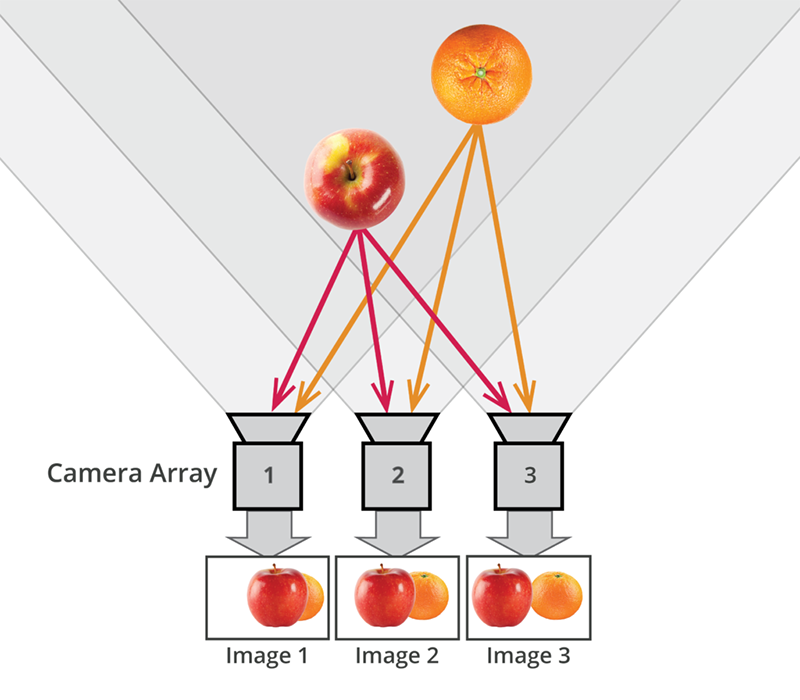
\includegraphics{img/what-is-a-light-field-disparity-recording-lytro.png}
    \caption{Cattura di un ligth field}
    \label{fig:ligthFieldRecording}
\end{figure}
\\
\\
I light field possono essere catturati utilizzando diverse tecniche, tra cui:
\begin{itemize}
    \item una singola telecamera controllata roboticamente,
    \item un arco rotante di telecamere,
    \item una serie di telecamere o moduli telecamere,
    \item una singola fotocamera dotata di un array di microlenti.
\end{itemize}

A seconda della tecnica utilizzata, i dati dell'immagine acquisita sono tipicamente costituiti da un’immagine contenente molte immagini secondarie (ottenute da un singolo sensore e una matrice di microlenti) o molte immagini (da più fotocamere o esposizioni). 
Entrambi i set di dati mostrano immagini con leggere variazioni, poiché catturano raggi di luce da diverse angolazioni nello spazio. Queste variazioni permettono di determinare la posizione degli oggetti e di creare un volume di campo luminoso 3D. Tuttavia, le fotocamere plenottiche come Lytro e Raytrix, sebbene offrano nuove opportunità, richiedono una compressione efficace per gestire le dimensioni considerevoli delle immagini raw e la loro rappresentazione non convenzionale, mantenendo al contempo la qualità dell'immagine.
\begin{figure}[ht!]
    \centering
    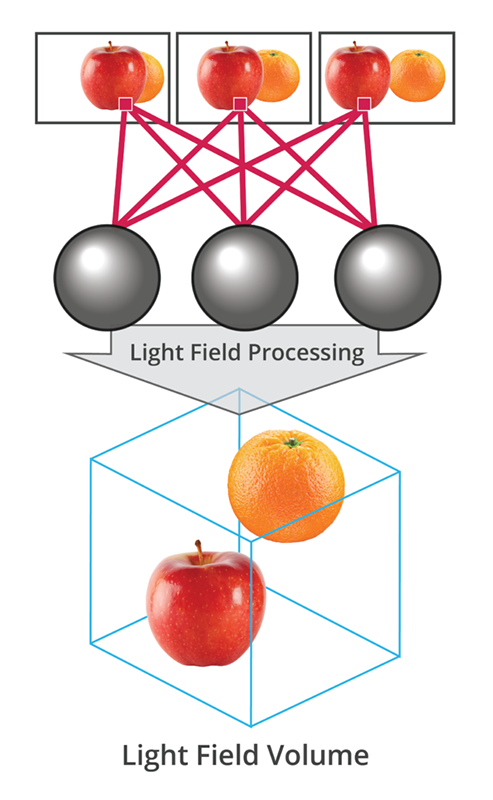
\includegraphics{img/what-is-a-light-field-disparity-processing-lytro.png}
    \caption{Informasioni racchiuse in un ligth field}
    \label{fig:ligthFieldInfo}
\end{figure}


\chapter{Lavori correlati}

Per la compressione dei ligth field ci siamo rifatti allo studio di un progetto passato svolto da nostri colleghi nell'università di Salerno\cite{LigthFieldCompression}.
\\
\\
I loro risulati si basano sulla compressione dei light field (che sono rappresentati tramite una serie immagini) in file di tipo video, così da sfruttare vari codec che si usano per comprimere le immagini in video.
\\
Precisamente i nostri colleghi hanno utilizzato i seguenti codec:
\begin{itemize}
    \item HVEC (lossy e lossless)
    \item VP9 (lossy e lossless)
    \item AV1 (lossy e lossless)
    \item HuffYUV (lossless)
    \item UT Video (lossless)
    \item FFV1 (lossless)
\end{itemize}
La nostra idea è quella di proseguire la strategia che i nostri colleghi hanno proposto andando ad espandere il loro studio già presente.



\chapter{Fase di ricerca}

Parte della ricerca si è basata sullo studio degli algoritmi utilizzati, e precisamente:
\begin{itemize}
    \item perché e quando sono stati creati,
    \item da chi sono stati prodotti,
    \item a quali bisogni rispondono,
    \item da chi sono stati utilizzati nel tempo.
\end{itemize}
Inoltre, è stato condotto un esperimento per determinare se vi fosse una dipendenza effettiva tra i vari frame dei light field e se tale dipendenza potesse influenzare la qualità complessiva della compressione/decompressione.
\\
Infine, è stata preparata una tabella riassuntiva per evidenziare le peculiarità fondamentali per la comprensione dei risultati del progetto. Ulteriormente, sono stati esaminati il Structural Similarity Index (SSIM) e il Peak Signal-to-Noise Ratio (PSNR), due metodi utilizzati per valutare la qualità percepita delle immagini in scenari di compressione lossy.

\clearpage
\section{Tabella riassuntiva}
\begin{table}[ht]
    \centering
     \begin{tabular}{|c|c|c|}
        \hline
        Codec & Licenza & Perdita \\
        \hline
        Cirrus Logic & Commerciale & Lossy \\
        FLV & GNU & Lossy \\
        MJPEG & GNU & Lossy \\
        MPEG4 & GNU & Lossy \\
        ProRes & Commerciale & Lossy \\
        \hline
        FFVHUFF & GNU & Lossless \\
        LCL-ZLIB & GNU & Lossless \\
        MAGICYUV & Commerciale & Lossless \\
        \hline
    \end{tabular}
    \label{tab:RecapTable}
\end{table}

\subsection{Cirrus Logic AccuPak}
Cirrus Logic AccuPak è un codec YUV a precisione ridotta.
\\
\\
Il codec AccuPak racchiude 4 campioni Y e 2 campioni C in 32 bit rappresentando ogni campione Y con 5 bit e ogni campione C con 6 bit. È essenzialmente un metodo ridimensionato di codifica YUV 4:1:1, in cui ogni gruppo di 4 pixel su una linea è rappresentato da un campione di luminanza ciascuno ma condivide campioni C\cite{CirrusLogicAccuPak}.

\subsection{FLV}
Flash Video è un formato di file utilizzato per fornire contenuti video digitali (ad esempio, programmi TV, film, ecc.) su Internet utilizzando Adobe Flash Player versione 6 e versioni più recenti. Il contenuto Flash Video può anche essere incorporato nei file SWF. Ci sono due diversi formati di file Flash Video: FLV e F4V. I dati audio e video all'interno dei file FLV sono codificati allo stesso modo dei file SWF. FLV è stato originariamente sviluppato da Macromedia. Nei primi anni 2000, Flash Video era lo standard de facto per lo streaming video basato sul web (su RTMP).
\\
\\
I file Flash Video FLV di solito contengono materiale codificato con codec che seguono i formati di compressione video Sorenson Spark o VP6. A partire dal 2010 le versioni pubbliche di Flash Player (collaborazione tra Adobe Systems e MainConcept) supportano anche il video H.264 e l'audio HE-AAC. Tutti questi formati di compressione sono limitati dai brevetti. Flash Video è visualizzabile sulla maggior parte dei sistemi operativi tramite Adobe Flash Player e il plugin del browser web o uno dei numerosi programmi di terze parti. I dispositivi iOS di Apple, insieme a quasi tutti gli altri dispositivi mobili, non supportano il plugin Flash Player e quindi richiedono altri metodi di consegna come quelli forniti da Adobe Flash Media Server\cite{FLV}.

\subsection{Motion JPEG}
Motion JPEG (M-JPEG) è un codec video nel quale ogni singolo frame del video viene compresso in un'immagine JPEG.
\\
Non offre nessuna compressione interframe, questo fa sì che la qualità della compressione sia indipendente dal movimento presente nell'immagine, a differenza della compressione MPEG dove ci possono essere problemi di qualità quando il video contiene movimenti veloci o cambi scena. Questo codec facilita il montaggio video, in quanto permette tagli su ogni singolo frame, e non solo all'inizio di un gruppo di frame.
\\
Si tratta di un formato che ha avuto una certa diffusione su fotocamere digitali e camere IP in quanto permetteva di usare la tecnologia della compressione JPEG anche per i filmati. Pur richiedendo un bitrate superiore al formato MPEG-1 permette risoluzioni superiori. È stato gradualmente soppiantato dai formati MOV(Apple), MPEG-2 e MPEG-4\cite{M-JPEG}.

\subsection{MPEG4}
In elettronica e telecomunicazioni MPEG-4, nato nel 1996 e finalizzato nel 1998 (fu presentato pubblicamente a settembre di quell'anno), è il nome dato a un insieme di standard per la codifica dell'audio e del video digitale sviluppati dall'ISO/IEC Moving Picture Experts Group (MPEG). L'MPEG-4 è uno standard utilizzato principalmente per applicazioni come la videotelefonia e la televisione digitale, per la trasmissione di filmati via Web, e per la memorizzazione su supporti CD-ROM.
\\
MPEG-4 è suddiviso in vari sotto standard chiamati part (termine inglese che in italiano significa "parte") e noi abbiamo usato la parte 2: un codec di compressione per i dati visivi (video, still textures...). Uno dei tanti "profili" della parte 2 è il Advanced Simple Profile (ASP).
\\
\\
Il concetto alla base del codec (COdificatore-DECodificatore) MPEG-4 è la quantizzazione. Senza scendere nello specifico, si può riassumere come quel processo che permette di trasmettere solamente la variazione dell'immagine mediante un apposito algoritmo di compressione\cite{MPEG-4}.

\subsection{ProRes}
Apple ProRes è un formato di compressione video lossy di alta qualità, "visually lossless" sviluppato da Apple Inc. per l'uso in post-produzione che supporta una risoluzione video fino a 8K. È il successore dell'Apple Intermediate Codec ed è stato introdotto nel 2007 con Final Cut Studio 2. Proprio come gli standard H.26x e MPEG, la famiglia di codec ProRes utilizza algoritmi di compressione basati sulla trasformata del coseno discreto (DCT). ProRes è ampiamente utilizzato come metodo di consegna del formato finale per i file di trasmissione HD in pubblicità, funzionalità, Blu-ray e streaming.
\\
\\
ProRes è una linea di codec intermedi, il che significa che sono destinati all'uso durante l'editing video e non alla visualizzazione pratica da parte dell'utente finale. Ciò si ottiene utilizzando solo la compressione intra-frame, dove ogni fotogramma viene memorizzato in modo indipendente e può essere decodificato senza dipendenze da altri fotogrammi. Il vantaggio di un codec intermedio è che offre eccellenti prestazioni di accesso casuale nelle applicazioni di post-produzione e mantiene una qualità superiore rispetto ai codec dell'utente finale, pur richiedendo sistemi disco molto meno costosi rispetto ai video non compressi. È paragonabile al codec DNxHD o CineForm di Avid che offrono bitrate simili e sono anche destinati ad essere utilizzati come codec intermedi. ProRes è un codec solo intra-frame basato su scalare DCT ed è quindi più semplice da decodificare rispetto ai formati orientati alla distribuzione come H.264. Nel 2018 Apple ha aggiunto un nuovo "ProRes RAW" (filtro Bayer compresso) a Final Cut Pro X, dopo che Blackmagic Design ha implementato Bayer compresso come "CinemaDNG 3:1" e "CinemaDNG 4:1" nelle loro fotocamere e DaVinci Resolve\cite{ProRes}.


\subsection{FFVHUFF}
FFVHUFF è un codec video senza perdita di dati ed è una versione migliorata, e più veloce, del codec huffyuv. Può gestire più formati pixel\cite{ffvhuff}.

\subsection{LCL-ZLIB}
Il codec converte i dati dell'immagine RGB24 originali in uno spazio colore di destinazione e lo comprime con un algoritmo selezionato. Il codec può anche rimuovere i fotogrammi invariati e sostituirli con fotogrammi nulli e può filtrare i dati dell'immagine prima della compressione. L'unica differenza tra avimszh e avizlib è nel compressore di flusso. Il filtraggio PNG è disponibile solo in avizlib. Fatta eccezione per i frame nulli, non c'è compressione temporale, e tutti i frame possono essere decodificati indipendentemente dagli altri. Ogni blocco AVI contiene un fotogramma. In caso di modalità multithread, le due sezioni sono memorizzate nello stesso blocco.
\\
Come suggerisce il nome del codec, tutti i compressori sono lossless.
\\
Questa modalità utilizza il metodo standard di sgonfiamento zlib. Per la descrizione dell'algoritmo fare riferimento ai documenti zlib. Lo stato del compressore viene reimpostato ogni fotogramma (decodifica ogni fotogramma in modo indipendente). I codici di compressione (1, 9, -1) hanno lo stesso significato dei flag di compressione zlib. Zlib non richiede un livello di compressione al decompressore, quindi il valore è lì solo a scopo informativo\cite{zlib}.

\subsection{MagicYuv}
Un codec video ad alte prestazioni, ultraveloce e matematicamente senza perdite per la registrazione, l'archiviazione, la post-produzione e l'editing ad alte risoluzioni.
\\
MagicYUV è stato progettato per la velocità e per supportare pienamente la codifica e la decodifica multi-thread.
\\
Questo codec è utilizzato per:
\begin{itemize}[noitemsep]
    \item Gaming
    \item Registrazioni e catture
    \item Editing e post-produzione
    \item Ricerca
\end{itemize}
Il Codec MagicYUV consente ai ricercatori di catturare ed elaborare video alle più alte risoluzioni e framerate possibili, in profondità di bit regolari e a colori profondi, mantenendo intatta ogni bit delle informazioni.
\\
Questo rende MagicYUV uno dei codec video lossless più veloci del suo genere\cite{magicyuv}.


\section{Metriche selezionate per il confronto}

\subsection{SSIM}
L'indice SSIM (Structural Similarity Index Measure) è un modello basato sulla percezione che valuta la degradazione dell'immagine considerando i cambiamenti nella percezione delle informazioni strutturali. Questo metodo tiene conto di importanti fenomeni basati sulla percezione, come il mascheramento della luminanza e il mascheramento del contrasto. Il termine "informazioni strutturali" si riferisce ai pixel fortemente interdipendenti o spazialmente vicini, enfatizzando la correlazione tra di essi.
SSIM stima la qualità percepita di immagini e video. Misura la somiglianza tra due immagini: l'originale e la recuperata\cite{sara2019image}.

In particolare, date due immagini o segnali $N$-dimensionali (o porzioni corrispondenti), $x = (x_1, \ldots, x_N)$ e $y = (y_1, \ldots, y_N)$, l'indice SSIM esamina le similarità tra luminanza, contrasto e struttura.

1. Per la luminanza, $l(x, y)$, si utilizzano i valori medi, ad esempio,
\[
\bar{x} = \frac{1}{N} \sum_{i=1}^{N} x_i.
\]

2. Per il contrasto, $c(x, y)$, si utilizzano le varianze, ad esempio,
\[
s_x^2 = \frac{1}{N-1} \sum_{i=1}^{N} (x_i - \bar{x})^2.
\]

3. Per la struttura, $s(x, y)$, si utilizzano segnali normalizzati (deviazione standard unitaria), ad esempio,
\[
x' = \frac{x - \bar{x}}{s_x}.
\]

Successivamente, si combinano questi componenti (in qualche modo!) per ottenere una misura complessiva di similarità, cioè,
\[
S(x, y) = F(l(x, y), c(x, y), s(x, y)).
\]

\subsection{PSNR}
Il PSNR (Peak Signal-to-Noise Ratio) è una metrica utilizzata per calcolare il rapporto tra la potenza massima del segnale possibile e la potenza del rumore di distorsione che influisce sulla qualità della sua rappresentazione. Questo rapporto tra due immagini viene misurato in decibel per tener conto della vasta gamma dinamica dei segnali, che variano dai valori più grandi a quelli più piccoli.
Il PSNR viene comunemente calcolato come il logaritmo in scala decibel, poiché i segnali hanno una gamma dinamica estesa. Questa gamma dinamica riflette la variazione tra i valori più alti e più bassi possibili, che sono critici per valutare la qualità dell'immagine in termini di fedeltà alla sua rappresentazione originale.
Utilizzato ampiamente come tecnica di valutazione della qualità, il PSNR misura la qualità della ricostruzione nei codec di compressione delle immagini lossy. In questo contesto, il segnale rappresenta i dati originali, mentre il rumore è l'errore introdotto dalla compressione o dalla distorsione. 
\\
\\
Nel degrado della qualità della compressione dell'immagine e del video, il valore PSNR varia da 30 a 50 dB per la rappresentazione dei dati a 8 bit e da 60 a 80 dB per i dati a 16 bit.
\\
\\
Il PSNR è espresso come:
\\
\centerline{$PSNR = 10log_{10}(peakval^2) / MSE$}
\\
\\
Qui, peakval (Peak Value) è il massimo nei dati dell'immagine. Se si tratta di un tipo di dati intero senza segno a 8 bit, il peakval è 255. Dall'equazione, possiamo vedere che è una rappresentazione dell'errore assoluto in dB\cite{sara2019image}.

\begin{figure}[!ht]
    \centering
    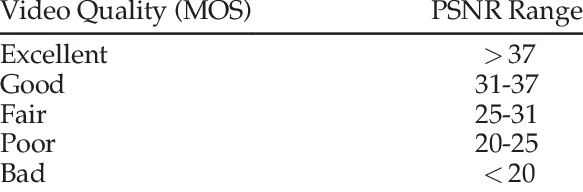
\includegraphics[width=0.40\textwidth]{img/PSNR table.png}
    \caption{Rapporto tra PSNR e qualità del video}
    \label{fig:PSNR-table}
\end{figure}


Nel paper "Social-Aware Video Multicast Based on Device-to-Device Communications" \cite{Social-Aware}, viene condotto uno studio che esamina il rapporto tra la qualità del video e il valore dell'indice PSNR. La Tabella \ref{fig:PSNR-table} fornisce una guida per interpretare i valori di PSNR e associarli a diverse categorie di qualità video. In particolare, si osserva che una qualità del video superiore è indicata da valori di PSNR pari o superiori a 37, mentre una qualità inferiore è associata a valori di PSNR inferiori a 25.
\\
\\
Nella fase di analisi dei risultati, la Tabella \ref{fig:PSNR-table} sarà utilizzata come riferimento per valutare la qualità dei video decompressi. In altre parole, i valori ottenuti durante l'esperimento saranno confrontati con i range indicati nella tabella per determinare se la qualità del video è considerata ottima, buona, accettabile o pessima, in base ai criteri definiti dagli intervalli di PSNR.

\subsection{Test indice SSIM con riferimento}
Per valutare l'accuratezza del calcolo dell'indice di similarità strutturale (SSIM) nel nostro lavoro, è stato condotto un confronto con i valori riportati nel paper di riferimento \textit{"The SSIM Index for Image Quality Assessment"} \cite{TEST_SSIM}. A tale scopo, le stesse immagini utilizzate nel paper di riferimento sono state scaricate e utilizzate per il calcolo dell'indice SSIM mediante uno script personalizzato basato sulla libreria \textit{skimage.metrics}. I valori ottenuti da questo script sono stati quindi confrontati con quelli riportati nel paper di riferimento.
\subsubsection{Risultati}
Il confronto tra i valori SSIM ottenuti dal nostro script e quelli riportati nel paper di riferimento ha mostrato una buona corrispondenza tra i due. Tuttavia, è stato osservato un errore medio relativo, calcolato come la media delle differenze percentuali tra i valori calcolati e quelli di riferimento, pari a \textbf{0.030}.
Questo risultato suggerisce che il nostro script per il calcolo dell'indice SSIM ha una precisione accettabile e può essere considerato affidabile per valutazioni quantitative della qualità delle immagini.

\subsection{Test indice PSNR con riferimento}
Per valutare l'accuratezza del calcolo del PSNR, sono state selezionate due immagini - l'originale e quella con rumore - estratte dalla pagina web specificata \cite{PSNR-HVS}, la quale fa riferimento a due paper accademici. Successivamente, utilizzando le informazioni fornite in questi paper, il PSNR è stato calcolato per le due immagini mediante l'utilizzo di uno script apposito che testa la funzione per il calcolo del PSNR fornita dalla libreria \textit{skimage.metrics} e usata nell'esperimento.

\subsubsection{Risultati}
I valori del PSNR ottenuti sono stati confrontati con quelli riportati sulla pagina web di riferimento, che fornisce i valori di PSNR associati alle immagini specificate. Questo confronto ha permesso di determinare l'errore relativo del PSNR, risultato essere dello 0.026\%. Questo risultato indica che vi è una buona corrispondenza tra i valori calcolati utilizzando la funzione di calcolo del PSNR fornita dalla libreria skimage.metrics e quelli riportati sulla pagina web di riferimento, confermando l'accuratezza del calcolo del PSNR.


\chapter{Sistema proposto}
Il nostro sistema ha come scopo principale quello di fornire un confronto tra vari algoritimi di compressione video e analizzare le loro prestazioni nella compressione di light field.
\\
Sostanzialmente, il nostro sistema è progettato per migliorare ed espandere uno studio precedente.
\\
\\
Come detto nel capitolo 3, le light field image hanno una forte componente di similarità tra frame della stessa scena. Si è deciso di sfruttare l’alta inter-dipendenza tra le varie immagini proprio come si fa per i video. 
\\
A tal fine abbiamo ri-implementato due script Python diversi, uno per la compressione dei light field in video e l’altro per la decompressione del video nelle sue componenti. Per la compressione usiamo diversi codec video, tutti di tipo lossless e lossy.

Per la decompressione invece usiamo il video creato nelle fasi precedenti e ne estraiamo i singoli frame. I frame estratti vengono poi salvati nello stesso formato delle immagini originali per monitorare così eventuali perdite di dati. Per ogni algoritmo di compressione effettuiamo un’analisi dello spazio risparmiato tramite il confronto della dimensione totale del dataset non compresso e del video compresso. Confrontiamo ogni frame decompresso con il suo corrispettivo originale, usando la structural similarity index measure (SSIM), per verificare che tra le due versioni non ci sia stata una perdita di informazioni nel caso di algoritmi lossless e che la perdita sia ”accettabile” per gli algoritmi lossy.
\\
\\
I vari processi verranno spiegati nel dettaglio al capitolo 6.
 


\chapter{Implementazione}

\section{Linguaggio, librerie principali e tool usati}
Per la realizzazione di questo progetto, è stato impiegato il linguaggio di programmazione Python (versione 3.11.6), facendo uso delle seguenti librerie:

\begin{enumerate}
    \item \textbf{Subprocess (versione 3.8):} La libreria subprocess è stata utilizzata per generare nuovi processi, connettersi alle loro pipe di input/output/errore e ottenere i relativi codici di ritorno;
    \item \textbf{FFmpeg (versione 6.1):} FFmpeg è una completa suite software nata nel dicembre 2000, specializzata in registrazione, conversione e riproduzione di audio e video. Basata sulla libreria libavcodec per la codifica audio/video, FFmpeg è sviluppata principalmente su Linux, ma può essere compilata ed eseguita su vari sistemi operativi, compreso Microsoft Windows. In particolare, l'uso di FFmpeg in questo contesto è stato orientato alla conversione video da un formato all'altro attraverso uno strumento da riga di comando.
    \item \textbf{OpenCV (opencv-python==4.8.1.78):} OpenCV è una libreria open-source che fornisce un'ampia varietà di strumenti per la visione artificiale e il machine learning. Nell'implementazione, OpenCV (cv2) è utilizzata per le operazioni di elaborazione delle immagini e manipolazione dei frame video.
    \item \textbf{CSV (csv):} La libreria csv inclusa in Python che offre funzionalità per la lettura e la scrittura di file CSV (Comma-Separated Values). Nell'implementazione è stata impiegata per la gestione per registrare risultati e statistiche del processo.
    \item \textbf{Scikit-image (scikit-image==0.22.0):} Scikit-image è una raccolta di algoritmi per il processamento delle immagini basata su Scikit-Learn. Le funzioni \textbf{structural\_similarity (ssim)} e \textbf{peak\_signal\_noise\_ratio (psnr)} fornite da skimage.metrics sono utilizzate per calcolare le metriche di similarità strutturale e rapporto segnale-rumore, rispettivamente.
\end{enumerate}

\section{Organizzazione del progetto e codice}

\subsection{Moduli python principali}
\begin{itemize}
    \item \textit{test\_compression.py:} Contiene funzioni e logica per la compressione video sui dataset presenti nel file utils.py.
    \item \textit{test\_decompression.py:} Gestisce la decompressione dei video compressi.
    \item \textit{utils.py:} Contiene funzioni di utilità condivise, nel nostro caso sono presenti i dataset testati, le estensioni corrette dei codec video e le cartelle di output per la compressione e la decompressione.
    \item \textit{random\_dataset.py:} lo scopo di questo script è randomizzare l'ordine dei file corrispondenti al pattern nella cartella di origine e copiarli in modo ordinato nella cartella di destinazione.
\end{itemize}

\subsection{Directory principali}
\begin{itemize}
    \item \textit{/datasets:} Contiene i dataset di input, in particolare ogni sottocartella fa riferimento ad uno specifico dataset.
    \item \textit{/compressione\_test:} Salva i risultati della compressione in una cartella contenente una sottocartella per ogni dataset. Ognuna di queste sottocartelle contiene a seconda dei codec usati il video compresso corrispondente. La seguente cartella in fase di compressione è creata in automatico.
    \item \textit{/decompression\_test:} Salva i risultati della decompressione in una cartella contenente una sottocartella per ogni dataset: Ognuna di queste contiene a seconda dei codec usati un'altra sottocartella all'interno della quale sono salvate le immagini decompresse. La cartella in fase di decompressione è creata in automatico.
    \item \textit{/ffmpeg:} Nel caso di un sistema Windows, questa cartella è di fondamentale importanza in quanto contiene l'eseguibile di ffmpeg.

\end{itemize}

\section{Metodologie esperimento}
L'esperimento è stato automatizzato per semplificare il processo, trasformandolo in un processo di \textit{benchmarking automatico} sia durante la fase di compressione che durante quella di decompressione. 
Di conseguenza, il programma eseguirà automaticamente i test con vari codec e sui vari dataset prensenti nel file python \textit{utils.py}, senza richiedere un'interazione continua da parte dell'utente. Questo approccio è particolarmente utile per condurre test di benchmark o valutare le prestazioni di diversi algoritmi in modo efficiente.
Per lanciare il test di compressione è possibile usare il comando \textit{python test\_compression.py} all'interno della cartella, mentre per testare la decompressione \textit{python test\_decompression.py}.

\section{Fase di compressione}

In fase di compressione sono state utilizzate diverse funzioni le quali firme seguono il pattern comp\_\{codec\_scelto\} e implementano il processo di compressione video mediante l'utilizzo di un codec specificato tramite FFmpeg. Il procedimento può essere riassunto in termini generici:

\begin{enumerate}
    \item \textbf{Parametri di Input:}
    \begin{itemize}
        \item input\_path: Percorso del file video originale;
        \item output\_path: Percorso in cui verrà salvato il file video compresso.
    \end{itemize}
    \item \textbf{Calcolo delle dimensioni:} Viene calcolata la dimensione totale del file originale attraverso la somma delle dimensioni di tutti i file presenti nella stessa cartella del file originale.
    \item \textbf{Utilizzo di FFmpeg per la compressione:} Utilizzando la libreria subprocess, viene eseguito FFmpeg dalla riga di comando. Il comando FFmpeg include specifiche come il tasso di frame di input, il codec video da utilizzare, insieme ai percorsi del file di input e di output;
    \item \textbf{Calcolo del tempo di compressione:} Il tempo di inizio viene registrato prima della chiamata FFmpeg, e il tempo di fine viene registrato dopo il completamento della compressione. La durata totale del processo di compressione viene calcolata sottraendo il tempo di inizio da quello di fine.
    \item \textbf{Calcolo del rapporto di compressione:} Utilizzando una funzione ausiliaria, vengono ottenute la dimensione del file compresso e il rapporto di compressione $\frac{dimensione\;originale}{dimensione \;compressa}$;
    \item \textbf{Output:} Ogni funzione di questo tipo restituisce la dimensione iniziale, la dimensione finale, il rapporto di compressione e il tempo impiegato per la compressione. Inoltre nella cartella di output sarà possibile visualizzare il video ottenuto dalla compressione.
\end{enumerate}
 Questo approccio è flessibile e può essere adattato per eseguire test con diversi codec, contribuendo così alla valutazione delle prestazioni dei codec nel contesto dell'esperimento.

\section{Fase di decompressione}
In fase di decompressione di un particolare video, il procedimento generale è questo:

\begin{enumerate}
    \item \textbf{Ciclo di decompressione}: Questa è la fase più importante e principale della decompressione. Il codice itera attraverso ogni frame del video compresso usando la libreria av. Durante l'iterazione, i frame vengono decodificati e salvati come immagini in una nuova directory, corrispondente al nome del dataset;
    \item \textbf{Creazione della struttura di output:} Viene creata una nuova directory per l'output della decompressione per ogni dataset. All'interno di ciascuna directory, vengono create sotto-directory per ogni algoritmo di compressione utilizzato.
    \item \textbf{Applicazione di metriche di qualità:} Per ogni coppia di immagini decompresse (originale e compressa), vengono calcolate metriche di qualità quali SSIM e PSNR. Le metriche vengono calcolate tra ogni frame dell'immagine originale e del risultato della decompressione;
    \item \textbf{Raccolta e salvataggio dei risultati:} I risultati delle metriche vengono raccolti e salvati in una struttura dati, che include informazioni come il nome del dataset, l'algoritmo di compressione utilizzato, e le medie delle metriche SSIM e PSNR (poiché vi è un confronto 1:1 tra immagine originale e immagine decompressa). I risultati vengono inoltre salvati in un file CSV per un'ulteriore analisi o documentazione.

\end{enumerate}

\section{Studio codec Lossy a parità di SSIM}

Il file dataset\_options.py contiene un dizionario chiamato DATASET\_OPTIONS, che definisce le impostazioni di compressione per ciascun dataset considerato durante gli esperimenti condotti. Ogni chiave del dizionario rappresenta un dataset specifico, mentre i valori associati a ciascuna chiave sono sotto-dizionari che specificano le opzioni di compressione per i diversi codec lossy utilizzati.

Per ogni dataset, sono elencati i codec FLV1, MJPEG, ProRes e MPEG4, insieme ai rispettivi valori del parametro \textit{-q:v}\cite{ffmpeg} di ffmpeg utilizzati per regolare la qualità della compressione. Questi valori di qualità sono stati scelti in base ai risultati degli esperimenti condotti, tenendo conto dell'effetto sul rapporto di compressione e sulla qualità dell'immagine, valutata principalmente attraverso l'indice SSIM.

È importante notare che l'aumento del valore del parametro -q:v tende a diminuire l'indice SSIM, il che indica una riduzione della qualità dell'immagine a fronte di una maggiore compressione. Questo aspetto è stato preso in considerazione durante la selezione delle opzioni di compressione al fine di mantenere un indice SSIM stabile per ciascun dataset, consentendo così un confronto accurato delle prestazioni dei codec lossy.












\chapter{Esperimenti svolti}
Una serie di esperimenti è stata condotta al fine di valutare l'efficacia del sistema proposto nella compressione video applicata alle light field images.

\section{Applicazione del sistema proposto sui dataset utilizzati in precedenza}
Inizialmente sono stati eseguiti una serie di test utilizzando il nostro sistema per valutare le prestazioni dei dataset precedenti. Ciò ha consentito di ottenere una comprensione più approfondita delle dinamiche operative e dei risultati ottenuti dai nostri precedessori, permettendoci, inoltre, di identificare fino a quale punto il sistema precedente ha risposto alle esigenze previste.
L'obiettivo principali è stato quello di valutare con maggiore precisione l'efficacia delle metodologie utilizzate precedentemente e di identificare eventuali punti deboli o aree di miglioramento. 

\section{Studio sulla correlazione tra light field contigui}
Al fine di valutare l'impatto dell'ordine dei frames nei dataset originali, è stato condotto uno studio supplementare. Ogni dataset originale è stato sottoposto a un processo di trasformazione, generando così un nuovo dataset in cui i frames sono disposti in maniera casuale. 
L'obiettivo di questo studio è comprendere come la disposizione casuale dei frames influenzi le prestazioni e i risultati dei codec di compressione. Tale approccio è fondamentale per valutare la resilienza dei codec di compressione rispetto a variazioni nell'ordine temporale dei frames. 

\section{Aggiunta di nuovi codec e nuovi dataset}
La scelta di aggiungere nuovi codec e di sottoporre tutti i dataset, vecchi e nuovi, a un riesame completo è stata fondamentale per comprendere in maniera esaustiva come le nuove implementazioni influiscano sulle prestazioni complessive del sistema. Tale approccio ha consentito di identificare correlazioni significative tra le caratteristiche dei codec, la selezione del dataset e le performance globali, contribuendo a delineare un quadro completo delle dinamiche del sistema in esame.


\subsection{Dataset utilizzati}
Per il miglioramento dello studio già effettuato dai nostri colleghi, abbiamo deciso di utilizzare i 3 dataset implementati nel loro progetto, in modo da poterli testare su nuovi codec, in aggiunta a 7 ulteriori dataset. Lo scopo è di avere un confronto tra più dati, in modo da raggiungere risultati più accurati.
\\
\\
I dadaset aggiunti sono i seguenti:
\begin{itemize}
    \item Il dataset ”Messerschmitt”\cite{Messerschmitt}, realizzato dal MIT Media Lab, propone 25 immagini in formato .png rappresentanti scene renderizzate, Figura\ref{fig:Messerschmitt}. Esse mostrano modelli 3D di una vettura del marchio Messerschmitt  realizzati dallo Stanford University Computer Graphics Laboratory \cite{3Dscanrep}. Tutti i light fields hanno una risoluzione di 840 x 593 pixel.
    
    \item Il dataset ”Dice”\cite{Dice}, realizzato dal MIT Media Lab, propone 25 immagini in formato .png rappresentanti scene renderizzate, Figura \ref{fig:Dice}. Esse mostrano modelli 3D di dadi da gioco realizzati dallo Stanford University Computer Graphics Laboratory \cite{3Dscanrep}. Tutti i light fields hanno una risoluzione di 840 x 593 pixel.
    
    \item Il dataset ”Fish”\cite{Fish}, realizzato dal MIT Media Lab, propone 25 immagini in formato .png rappresentanti scene renderizzate, Figura \ref{fig:Fish}. Esse mostrano modelli 3D pesci realizzati dallo Stanford University Computer Graphics Laboratory \cite{3Dscanrep}. Tutti i light fields hanno una risoluzione di 840 x 593 pixel.

    \item  Il dataset ”Car”\cite{Car} realizzato dal Max Planck Institut Informatik. Esso consiste in 101 immagini in formato .png, rappresentanti scene renderizzate, Figura \ref{fig:Car}. Esse presentano scene 3D di una autovettura. Tutti i light fields hanno una risoluzione spaziale di 960 x 720 pixel

    \item  Il dataset ”Cobblestone”\cite{Cobblestone} realizzato dal Max Planck Institut Informatik. Esso consiste in 101 immagini in formato .png, rappresentanti scene renderizzate, Figura \ref{fig:Cobblestone}. Esse presentano scene 3D di un sentiero di pietra. Tutti i light fields hanno una risoluzione spaziale di 960 x 720 pixel

    \item  Il dataset ”Mannequin”\cite{Mannequin} realizzato dal Max Planck Institut Informatik. Esso consiste in 101 immagini in formato .png, rappresentanti scene renderizzate, Figura \ref{fig:Mannequin}. Esse presentano scene 3D di un manichino in una stanza. Tutti i light fields hanno una risoluzione spaziale di 960 x 720 pixel

    \item  Il dataset ”Blob”\cite{Blob} realizzato dal Max Planck Institut Informatik. Esso consiste in 101 immagini in formato .png, rappresentanti scene renderizzate, Figura \ref{fig:Blob}. Esse presentano scene 3D di un "blob". Tutti i light fields hanno una risoluzione spaziale di 960 x 720 pixel


\end{itemize}


\begin{figure}[ht]
    \centering
    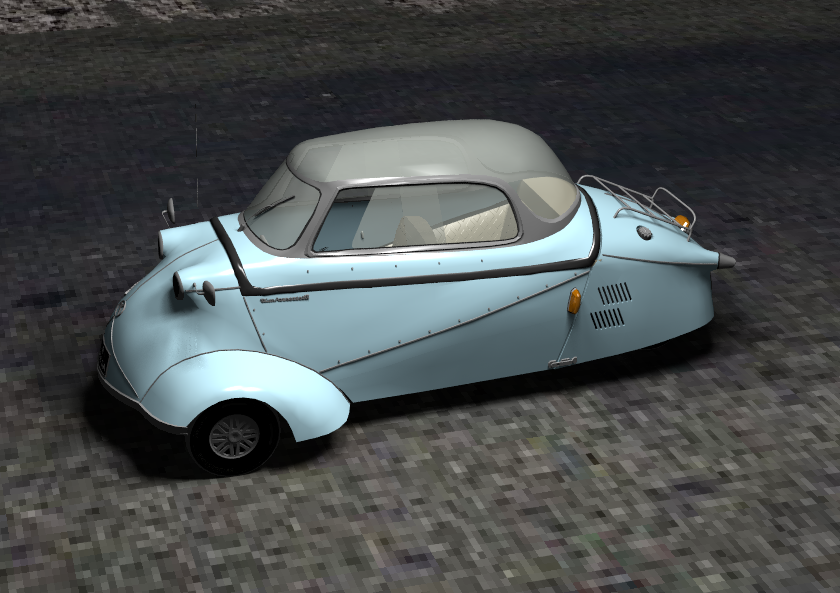
\includegraphics[width=0.5\textwidth]{img/Messerschmitt.png}
    \caption{Immagine estratta dal dataset ”Messerschmitt”}
    \label{fig:Messerschmitt}
\end{figure}

\begin{figure}[ht]
    \centering
    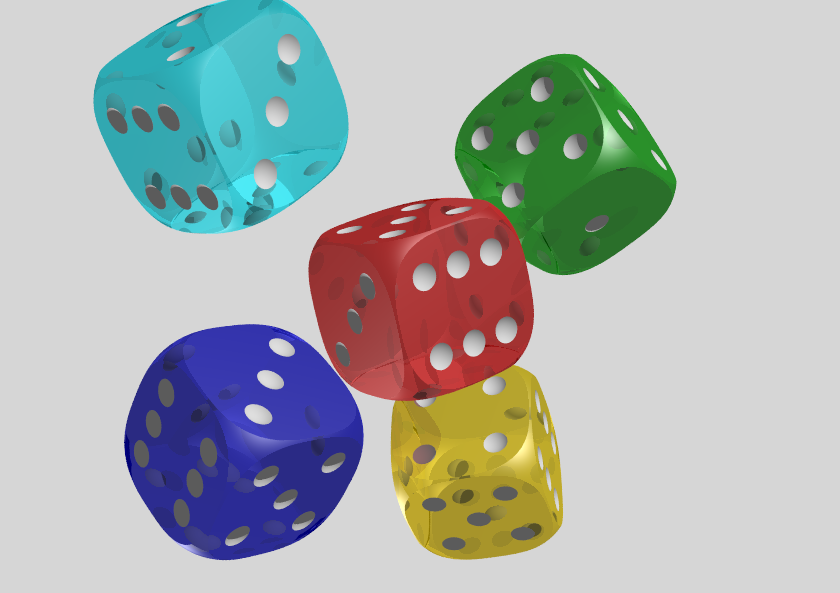
\includegraphics[width=0.5\textwidth]{img/Dice.png}
    \caption{Immagine estratta dal dataset ”Dice”}
    \label{fig:Dice}
\end{figure}

\begin{figure}[ht]
    \centering
    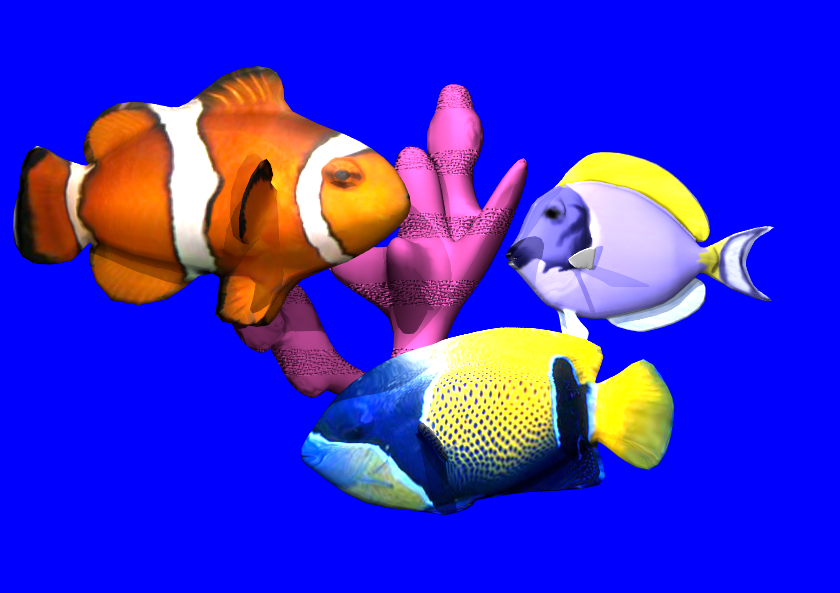
\includegraphics[width=0.5\textwidth]{img/Fish.png}
    \caption{Immagine estratta dal dataset ”Fish”}
    \label{fig:Fish}
\end{figure}

\begin{figure}[ht]
    \centering
    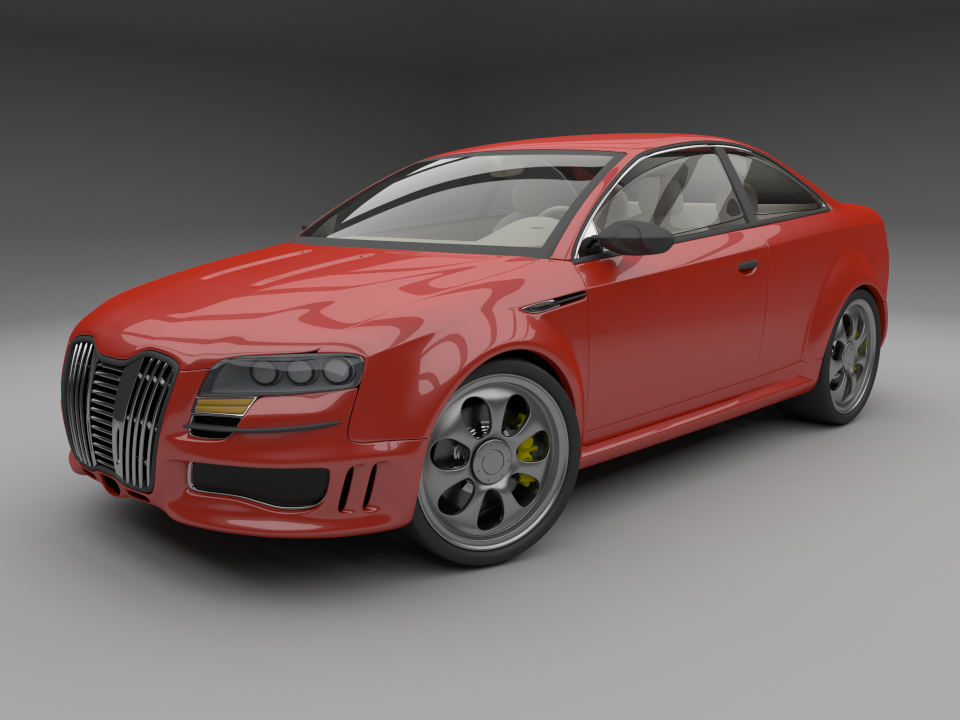
\includegraphics[width=0.5\textwidth]{img/Car.png}
    \caption{Immagine estratta dal dataset ”Car”}
    \label{fig:Car}
\end{figure}

\begin{figure}[ht]
    \centering
    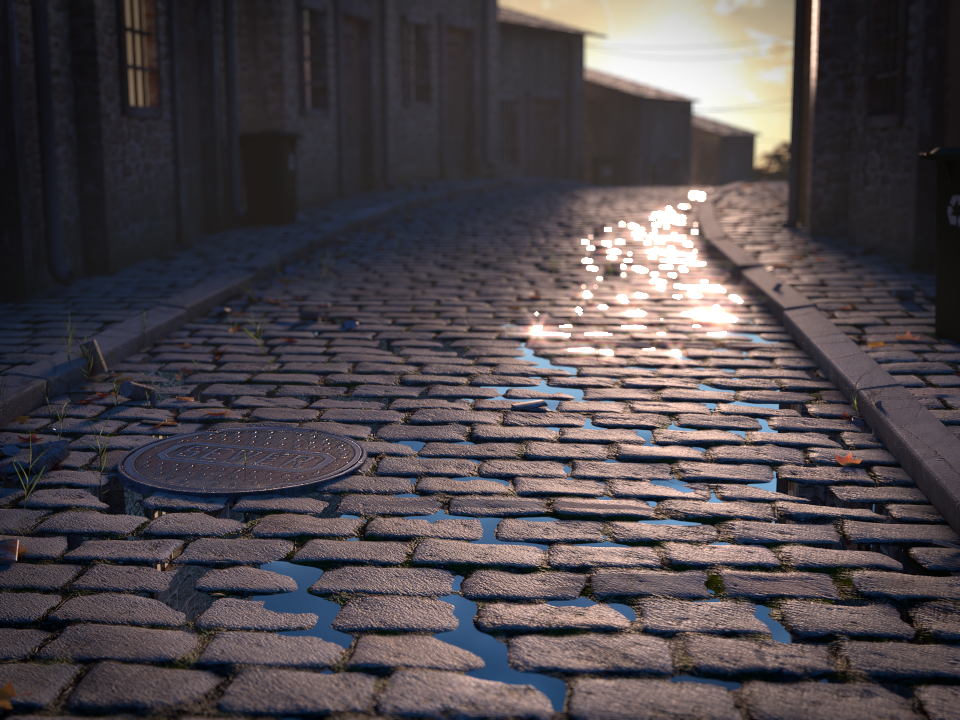
\includegraphics[width=0.5\textwidth]{img/Cobblestone.png}
    \caption{Immagine estratta dal dataset ”Cobblestone”}
    \label{fig:Cobblestone}
\end{figure}

\begin{figure}[ht]
    \centering
    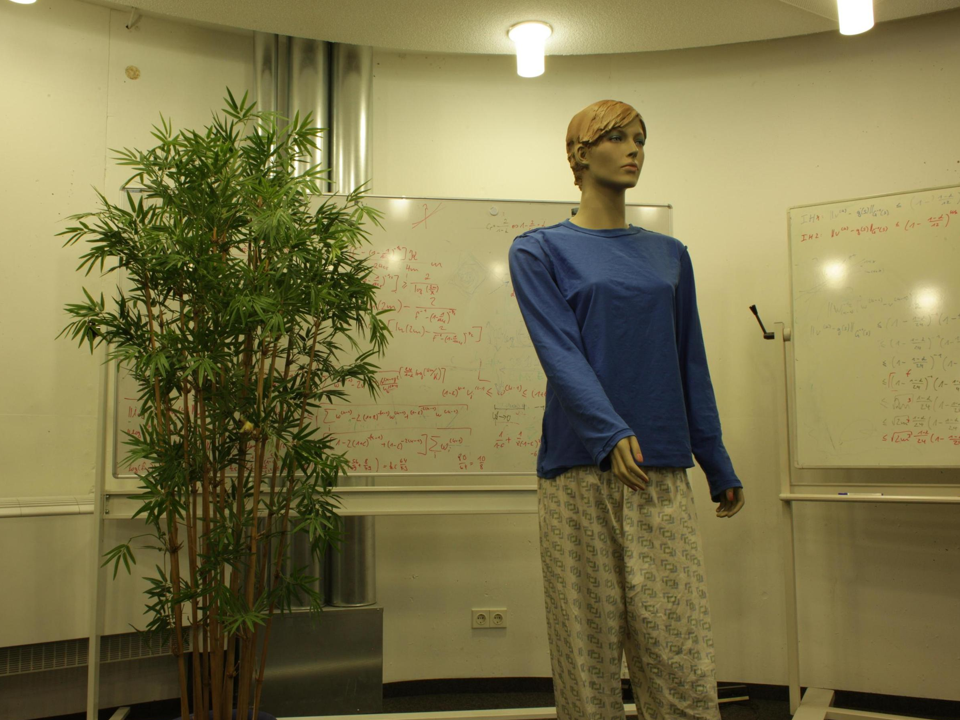
\includegraphics[width=0.5\textwidth]{img/Mannequin.png}
    \caption{Immagine estratta dal dataset ”Mannequin”}
    \label{fig:Mannequin}
\end{figure}

\begin{figure}[ht]
    \centering
    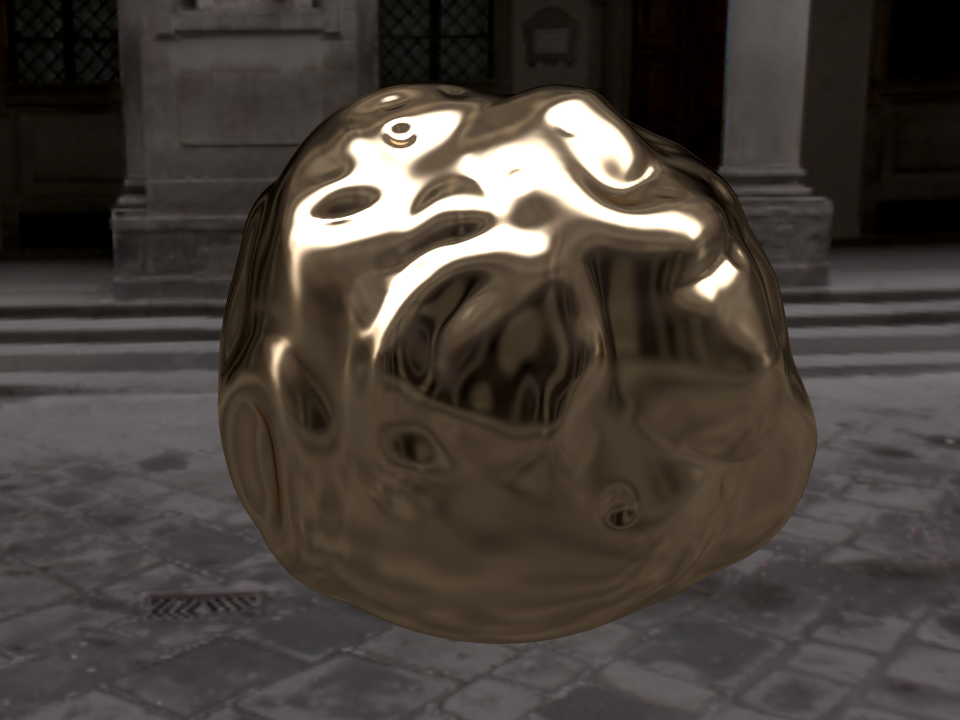
\includegraphics[width=0.5\textwidth]{img/Blob.png}
    \caption{Immagine estratta dal dataset ”Blob”}
    \label{fig:Blob}
\end{figure}
\clearpage



\chapter{Analisi dei risultati}
\section{Configurazione Hardware}
Gli esperimento sono stati condotti utilizzando una configurazione hardware di questo tipo:
\begin{itemize}
    \item processore Ryzen 5 2600;
    \item scheda grafica GTX 1660;
    \item  16 GB di RAM
\end{itemize}
Questa combinazione di componenti è stata scelta per garantire prestazioni affidabili e rappresentative nell'ambito delle attività di compressione.

\section{Nomenclatura esperimenti svolti}
Nel corso delle nostre ricerche e dei vari esperimenti condotti, abbiamo adottato diversi nomi per distinguere e identificare in modo chiaro i diversi aspetti delle nostre indagini. Per riferirci ai codec video e ai dataset forniti dai nostri stimati colleghi, abbiamo deciso di utilizzare l'anno 2022 come riferimento nei nomi degli esperimenti. 
\\
\\
Per quanto riguarda i dataset e i codec video scelti e utilizzati nei nostri studi, abbiamo adottato l'anno 2023 come punto di riferimento nei nomi assegnati a tali risorse. 
\clearpage
\section{Risultati ottenuti}
Di seguito riportiamo i vari esperimenti da noi proposti. Abbiamo scelto di dividere i risultati in vari esperimenti per avere una visione più completa sia sul lavoro sia dei nostri predecessori che sulle nostre proposte.
\\
Per ogni studio riportiamo una tabella che riassume tutti i dati dell'esperimento  che rappresenta visivamente l'andamento dei vari codec sui vari dataset.

\subsection{Codec 2022 sui dataset 2022}
Questo studio è stato svolto per testare nuovamente i risultati dei nostri predecessori per riconfermare i risultati dopo aver apportato modifiche al codice sorgente.
\\
\\
Di seguito riportiamo le tabelle (una per dataset) su questo studio:

\begin{table}[ht]
\begin{tabular}{|l|l|l|l|l|}
\hline
Dataset     & Algoritmo & \begin{tabular}[c]{@{}c@{}}Rapporto \\ compressione\end{tabular} & \begin{tabular}[c]{@{}c@{}}Tempo \\ compressione\end{tabular} & \begin{tabular}[c]{@{}c@{}}Dimensione \\ finale\end{tabular} \\ \hline
ArtGallery2 & HEVC      & 1.943                                               & 20.48s                                                        & 45927441                                                     \\ \hline
ArtGallery2 & VP9       & 1.645                                                & 33.54s                                                        & 54234262                                                     \\ \hline
ArtGallery2 & AV1       & 1.772                                               & 1791.34s                                                      & 50358098                                                     \\ \hline
ArtGallery2 & FFV1      & 1.365                                               & 1.96s                                                         & 65351370                                                     \\ \hline
ArtGallery2 & HUFFYUV   & 1.057                                               & 0.28s                                                         & 84401008                                                     \\ \hline
ArtGallery2 & UTVIDEO   & 1.089                                                & 0.36s                                                         & 81902122                                                     \\ \hline

\end{tabular}
\caption{Studio codec 2022 sul dataset "ArtGallery"}
\end{table}

\begin{table}[ht]
\begin{tabular}{|l|l|l|l|l|}
\hline
Dataset     & Algoritmo & \begin{tabular}[c]{@{}c@{}}Rapporto \\ compressione\end{tabular} & \begin{tabular}[c]{@{}c@{}}Tempo \\ compressione\end{tabular} & \begin{tabular}[c]{@{}c@{}}Dimensione \\ finale\end{tabular} \\ \hline
Dragons     & HEVC      & 1.804                                                & 3.55s                                                         & 6538887                                                      \\ \hline
Dragons     & VP9       & 1.450                                               & 10.27s                                                        & 8132950                                                      \\ \hline
Dragons     & AV1       & 1.514                                               & 251.60s                                                       & 7789378                                                      \\ \hline
Dragons     & FFV1      & 1.329                                               & 0.44s                                                         & 8875630                                                      \\ \hline
Dragons     & HUFFYUV   & 0.747                                               & 0.12s                                                         & 15779892                                                     \\ \hline
Dragons     & UTVIDEO   & 0.882                                               & 0.14s                                                         & 13369862                                                     \\ \hline
\end{tabular}
\caption{Studio codec 2022 sul dataset "Dragons and bunnies"}
\end{table}

\begin{table}[ht]
\begin{tabular}{|l|l|l|l|l|}
\hline
Dataset     & Algoritmo & \begin{tabular}[c]{@{}c@{}}Rapporto \\ compressione\end{tabular} & \begin{tabular}[c]{@{}c@{}}Tempo \\ compressione\end{tabular} & \begin{tabular}[c]{@{}c@{}}Dimensione \\ finale\end{tabular} \\ \hline
OpEx        & HEVC      & 1.130                                               & 47.13s                                                        & 65274281                                                     \\ \hline
OpEx        & VP9       & 1.094                                             & 56.67s                                                        & 67410595                                                     \\ \hline
OpEx        & AV1       & 1.240                                                & 2519.93s                                                      & 59501300                                                     \\ \hline
OpEx        & FFV1      & 1.596                                               & 7.92s                                                         & 46216186                                                     \\ \hline
OpEx        & HUFFYUV   & 0.424                                               & 5.35s                                                         & 173654640                                                    \\ \hline
OpEx        & UTVIDEO   & 0.676                                               & 5.19s                                                         & 109078914                                                    \\ \hline
\end{tabular}
\caption{Studio codec 2022 sul dataset "OpEx Room"}
\end{table}


\clearpage
\subsection{Codec 2022 sui dataset 2022 (random)}
Questo studio è stato svolto per testare i codec 2022 sui dataset 2022, però con i frame disposti in maniera casuale (random).
\\
\\
Di seguito riportiamo le tabelle (una per dataset)  su questo studio:

\begin{table}[ht]
\begin{tabular}{|l|l|c|c|c|}
\hline
Dataset             & Algoritmo & \begin{tabular}[c]{@{}c@{}}Rapporto \\ compressione\end{tabular} & \begin{tabular}[c]{@{}c@{}}Tempo \\ compressione\end{tabular} & \begin{tabular}[c]{@{}c@{}}Dimensione \\ finale\end{tabular} \\ \hline
ArtGallery2\_random & HEVC      & 1.385                                               & 24.83s                                                        & 64408395                                                     \\ \hline
ArtGallery2\_random & VP9       & 1.142                                               & 37.77s                                                        & 78145982                                                     \\ \hline
ArtGallery2\_random & AV1       & 1.457                                               & 1477.19s                                                      & 61221006                                                     \\ \hline
ArtGallery2\_random & FFV1      & 1.365                                               & 1.93s                                                         & 65370246                                                     \\ \hline
ArtGallery2\_random & HUFFYUV   & 1.057                                               & 0.27s                                                         & 84401008                                                     \\ \hline
ArtGallery2\_random & UTVIDEO   & 1.089                                                & 0.35s                                                         & 81902122                                                     \\ \hline
\end{tabular}
\caption{Studio codec 2022 sul dataset \textbf{random} "ArtGallery"}
\end{table}

\begin{table}[ht]
\begin{tabular}{|l|l|c|c|c|}
\hline
Dataset             & Algoritmo & \begin{tabular}[c]{@{}c@{}}Rapporto \\ compressione\end{tabular} & \begin{tabular}[c]{@{}c@{}}Tempo \\ compressione\end{tabular} & \begin{tabular}[c]{@{}c@{}}Dimensione \\ finale\end{tabular} \\ \hline
Dragons\_random     & HEVC      & 1.553                                              & 3.51s                                                         & 7595776                                                      \\ \hline
Dragons\_random     & VP9       & 1.310                                               & 11.40s                                                        & 9006578                                                      \\ \hline
Dragons\_random     & AV1       & 1.432                                               & 244.98s                                                       & 8234601                                                      \\ \hline
Dragons\_random     & FFV1      & 1.329                                               & 0.44s                                                         & 8878232                                                      \\ \hline
Dragons\_random     & HUFFYUV   & 0.747                                               & 0.11s                                                         & 15779892                                                     \\ \hline
Dragons\_random     & UTVIDEO   & 0.882                                               & 0.13s                                                         & 13369862                                                     \\ \hline
\end{tabular}

\caption{Studio codec 2022 sul dataset \textbf{random} "Dragons and bunnies"}
\end{table}

\begin{table}[ht]
\begin{tabular}{|l|l|c|c|c|}
\hline
Dataset             & Algoritmo & \begin{tabular}[c]{@{}c@{}}Rapporto \\ compressione\end{tabular} & \begin{tabular}[c]{@{}c@{}}Tempo \\ compressione\end{tabular} & \begin{tabular}[c]{@{}c@{}}Dimensione \\ finale\end{tabular} \\ \hline
OpEx\_random       & HEVC      & 1.001                                               & 54.78s                                                        & 73701921                                                     \\ \hline
OpEx\_random       & VP9       & 1.037                                               & 69.50s                                                        & 71118193                                                     \\ \hline
OpEx\_random       & AV1       & 1.161                                               & 2797.33s                                                      & 63524638                                                     \\ \hline
OpEx\_random       & FFV1      & 1.507                                               & 7.95s                                                         & 48967364                                                     \\ \hline
OpEx\_random        & HUFFYUV   & 0.393                                               & 5.64s                                                         & 187652124                                                    \\ \hline
OpEx\_random        & UTVIDEO   & 0.628                                               & 4.99s                                                         & 117380518                                                    \\ \hline
\end{tabular}
\caption{Studio codec 2022 sul dataset \textbf{random} "OpEx Room"}
\end{table}

\clearpage
\subsection{Codec 2022 sui dataset 2023}
Questo studio è stato svolto per testare i codec 2022 sui nuovi dataset 2023 implementati da noi. L'obiettivo dietro a questo esperimento è di ottenere una quantità maggiore di dati per avere un idea più completa sui codec 2022.
\\
\\
Di seguito riportiamo le tabelle (una per dataset) su questo studio:

\begin{table}[ht]
\begin{tabular}{|l|c|c|c|c|}
\hline
Dataset       & Algoritmo & \begin{tabular}[c]{@{}c@{}}Rapporto \\ compressione\end{tabular} & \begin{tabular}[c]{@{}c@{}}Tempo \\ compressione\end{tabular} & \begin{tabular}[c]{@{}c@{}}Dimensione \\ finale\end{tabular} \\ \hline
Blob          & HEVC      & 2.644                                               & 16.23s                                                        & 20286094                                                     \\ \hline
Blob          & VP9       & 1.123                                                & 46.23s                                                        & 47745505                                                     \\ \hline
Blob          & AV1       & 2.312                                                & 1425.33s                                                      & 23199679                                                     \\ \hline
Blob          & FFV1      & 1.642                                                & 1.46s                                                         & 32667866                                                     \\ \hline
Blob          & HUFFYUV   & 0.823                                               & 0.28s                                                         & 65166640                                                     \\ \hline
Blob          & UTVIDEO   & 1.002                                               & 0.36s                                                         & 53500422                                                     \\ \hline
\end{tabular}
\caption{Studio codec 2022 sul dataset "Blob"}
\end{table}

\begin{table}[ht]
\begin{tabular}{|l|c|c|c|c|}
\hline
Dataset       & Algoritmo & \begin{tabular}[c]{@{}c@{}}Rapporto \\ compressione\end{tabular} & \begin{tabular}[c]{@{}c@{}}Tempo \\ compressione\end{tabular} & \begin{tabular}[c]{@{}c@{}}Dimensione \\ finale\end{tabular} \\ \hline
Car           & HEVC      & 2.149                                               & 15.36s                                                        & 29547917                                                     \\ \hline
Car           & VP9       & 1.408                                               & 32.35s                                                        & 45082057                                                     \\ \hline
Car           & AV1       & 1.753                                               & 2647.55s                                                      & 36207643                                                     \\ \hline
Car           & FFV1      & 1.756                                                & 2.33s                                                         & 36146340                                                     \\ \hline
Car           & HUFFYUV   & 0.970                                               & 0.33s                                                         & 65438568                                                     \\ \hline
Car           & UTVIDEO   & 1.194                                               & 0.51s                                                         & 53141066                                                     \\ \hline
\end{tabular}
\caption{Studio codec 2022 sul dataset "Car"}
\end{table}

\begin{table}[ht]
\begin{tabular}{|l|c|c|c|c|}
\hline
Dataset       & Algoritmo & \begin{tabular}[c]{@{}c@{}}Rapporto \\ compressione\end{tabular} & \begin{tabular}[c]{@{}c@{}}Tempo \\ compressione\end{tabular} & \begin{tabular}[c]{@{}c@{}}Dimensione \\ finale\end{tabular} \\ \hline
Cobblestone   & HEVC      & 2.044                                               & 21.64s                                                        & 50287099                                                     \\ \hline
Cobblestone   & VP9       & 1.232                                               & 39.56s                                                        & 83437410                                                     \\ \hline
Cobblestone   & AV1       & 2.006                                             & 1597.50s                                                      & 51230047                                                     \\ \hline
Cobblestone   & FFV1      & 1.365                                                & 2.54s                                                         & 75263866                                                     \\ \hline
Cobblestone   & HUFFYUV   & 1.028                                               & 0.26s                                                         & 99919324                                                     \\ \hline
Cobblestone   & UTVIDEO   & 1.052                                                & 0.34s                                                         & 97681582                                                     \\ \hline
\end{tabular}
\caption{Studio codec 2022 sul dataset "Cobblestone"}
\end{table}

\begin{table}[ht]
\begin{tabular}{|l|c|c|c|c|}
\hline
Dataset       & Algoritmo & \begin{tabular}[c]{@{}c@{}}Rapporto \\ compressione\end{tabular} & \begin{tabular}[c]{@{}c@{}}Tempo \\ compressione\end{tabular} & \begin{tabular}[c]{@{}c@{}}Dimensione \\ finale\end{tabular} \\ \hline
Dice          & HEVC      & 1.007                                               & 2.93s                                                         & 3108647                                                      \\ \hline
Dice          & VP9       & 0.927                                               & 8.07s                                                         & 3376922                                                      \\ \hline
Dice          & AV1       & 0.990                                                & 95.82s                                                        & 3161975                                                      \\ \hline
Dice          & FFV1      & 1.447                                                & 0.22s                                                         & 2163376                                                      \\ \hline
Dice          & HUFFYUV   & 0.289                                               & 0.09s                                                         & 10826588                                                     \\ \hline
Dice          & UTVIDEO   & 0.469                                               & 0.11s                                                         & 6663838                                                      \\ \hline
\end{tabular}
\caption{Studio codec 2022 sul dataset "Dice"}
\end{table}

\begin{table}[ht]
\begin{tabular}{|l|c|c|c|c|}
\hline
Dataset       & Algoritmo & \begin{tabular}[c]{@{}c@{}}Rapporto \\ compressione\end{tabular} & \begin{tabular}[c]{@{}c@{}}Tempo \\ compressione\end{tabular} & \begin{tabular}[c]{@{}c@{}}Dimensione \\ finale\end{tabular} \\ \hline
Fish          & HEVC      & 2.109                                                 & 2.46s                                                         & 3487710                                                      \\ \hline
Fish          & VP9       & 1.726                                               & 5.93s                                                         & 4261923                                                      \\ \hline
Fish          & AV1       & 1.946                                               & 125.60s                                                       & 3780963                                                      \\ \hline
Fish          & FFV1      & 1.227                                               & 0.36s                                                         & 5992874                                                      \\ \hline
Fish          & HUFFYUV   & 0.518                                               & 0.12s                                                         & 14194972                                                     \\ \hline
Fish          & UTVIDEO   & 0.658                                               & 0.13s                                                         & 11167262                                                     \\ \hline
\end{tabular}
\caption{Studio codec 2022 sul dataset "Fish"}
\end{table}

\begin{table}[ht]
\begin{tabular}{|l|c|c|c|c|}
\hline
Dataset       & Algoritmo & \begin{tabular}[c]{@{}c@{}}Rapporto \\ compressione\end{tabular} & \begin{tabular}[c]{@{}c@{}}Tempo \\ compressione\end{tabular} & \begin{tabular}[c]{@{}c@{}}Dimensione \\ finale\end{tabular} \\ \hline
Mannequin     & HEVC      & 1.099                                                & 25.17s                                                        & 72752630                                                     \\ \hline
Mannequin     & VP9       & 1.085                                               & 40.57s                                                        & 73663937                                                     \\ \hline
Mannequin     & AV1       & 1.263                                               & 1962.75s                                                      & 63306464                                                     \\ \hline
Mannequin     & FFV1      & 1.561                                               & 1.70s                                                         & 51220344                                                     \\ \hline
Mannequin     & HUFFYUV   & 0.921                                               & 0.28s                                                         & 86783324                                                     \\ \hline
Mannequin     & UTVIDEO   & 0.996                                               & 0.41s                                                         & 80218574                                                     \\ \hline
\end{tabular}
\caption{Studio codec 2022 sul dataset "Mannequin"}
\end{table}

\begin{table}[ht]
\begin{tabular}{|l|c|c|c|c|}
\hline
Dataset       & Algoritmo & \begin{tabular}[c]{@{}c@{}}Rapporto \\ compressione\end{tabular} & \begin{tabular}[c]{@{}c@{}}Tempo \\ compressione\end{tabular} & \begin{tabular}[c]{@{}c@{}}Dimensione \\ finale\end{tabular} \\ \hline
Messerschmitt & HEVC      & 1.370                                               & 4.02s                                                         & 6462662                                                      \\ \hline
Messerschmitt & VP9       & 0.973                                              & 11.24s                                                        & 9101952                                                      \\ \hline
Messerschmitt & AV1       & 1.089                                                & 201.96s                                                       & 8127707                                                      \\ \hline
Messerschmitt & FFV1      & 1.720                                               & 0.37s                                                         & 5149332                                                      \\ \hline
Messerschmitt & HUFFYUV   & 0.753                                               & 0.11s                                                         & 11756164                                                     \\ \hline
Messerschmitt & UTVIDEO   & 1.027                                               & 0.13s                                                         & 8617930                                                      \\ \hline
\end{tabular}
\caption{Studio codec 2022 sul dataset "Messerschmitt"}
\end{table}

\clearpage
\subsection{Codec 2022 sui dataset 2023 (random)}
Questo studio è stato svolto per testare i codec 2022 sui nuovi dataset 2023 implementati da noi andando a randomizzare i frames dei dataset scelti da noi per testare se c'è correlazione con lo studio precedente. 
\\
\\
Di seguito riportiamo le tabelle (una per dataset)  su questo studio:
\begin{table}[ht]
\centering
\begin{tabular}{|l|c|c|c|c|}
\hline
Dataset               & Algoritmo & \begin{tabular}[c]{@{}c@{}}Rapporto \\ compressione\end{tabular} & \begin{tabular}[c]{@{}c@{}}Tempo \\ compressione\end{tabular} & \begin{tabular}[c]{@{}c@{}}Dimensione \\ finale\end{tabular} \\ \hline
Blob\_random          & HEVC      & 1.681                                                & 19.63                                                         & 31917331                                                     \\ \hline
Blob\_random          & VP9       & 1.032                                               & 42.06s                                                        & 51991103                                                     \\ \hline
Blob\_random          & AV1       & 1.963                                               & 934.95s                                                       & 27323634                                                     \\ \hline
Blob\_random        & FFV1      & 1.641                                               & 1.71s                                                         & 32689958                                                     \\ \hline
Blob\_random          & HUFFYUV   & 0.823                                               & 0.28s                                                         & 65166640                                                     \\ \hline
Blob\_random          & UTVIDEO   & 1.002                                               & 0.36s                                                         & 53500422                                                     \\ \hline
\end{tabular}
\caption{Studio codec 2022 sul dataset \textbf{random} "Blob"}
\end{table}

\begin{table}[ht]
\centering
\begin{tabular}{|l|c|c|c|c|}
\hline
Dataset               & Algoritmo & \begin{tabular}[c]{@{}c@{}}Rapporto \\ compressione\end{tabular} & \begin{tabular}[c]{@{}c@{}}Tempo \\ compressione\end{tabular} & \begin{tabular}[c]{@{}c@{}}Dimensione \\ finale\end{tabular} \\ \hline
Car\_random           & HEVC      & 1.401                                               & 22.08s                                                        & 45307730                                                     \\ \hline
Car\_random           & VP9       & 1.010                                               & 41.80s                                                        & 62818936                                                     \\ \hline
Car\_random           & AV1       & 1.319                                               & 2314.73s                                                      & 48134236                                                     \\ \hline
Car\_random           & FFV1      & 1.755                                               & 1.51s                                                         & 36179160                                                     \\ \hline
Car\_random           & HUFFYUV   & 0.970                                               & 0.28s                                                         & 65438568                                                     \\ \hline
Car\_random           & UTVIDEO   & 1.194                                               & 0.37s                                                         & 53141066                                                     \\ \hline
\end{tabular}
\caption{Studio codec 2022 sul dataset \textbf{random} "Car"}
\end{table}

\begin{table}[ht]
\centering
\begin{tabular}{|l|c|c|c|c|}
\hline
Dataset               & Algoritmo & \begin{tabular}[c]{@{}c@{}}Rapporto \\ compressione\end{tabular} & \begin{tabular}[c]{@{}c@{}}Tempo \\ compressione\end{tabular} & \begin{tabular}[c]{@{}c@{}}Dimensione \\ finale\end{tabular} \\ \hline
Cobblestone\_random   & HEVC      & 1.387                                                & 20.03s                                                        & 74081960                                                     \\ \hline
Cobblestone\_random   & VP9       & 0.943                                               & 40.91s                                                        & 108910835                                                    \\ \hline
Cobblestone\_random   & AV1       & 1.601                                               & 1118.97s                                                      & 64174845                                                     \\ \hline
Cobblestone\_random   & FFV1      & 1.365                                               & 2.59s                                                         & 75277548                                                     \\ \hline
Cobblestone\_random   & HUFFYUV   & 1.028                                                & 0.29s                                                         & 99919324                                                     \\ \hline
Cobblestone\_random   & UTVIDEO   & 1.052                                                & 0.36s                                                         & 97681582                                                     \\ \hline
\end{tabular}
\caption{Studio codec 2022 sul dataset \textbf{random} "Cobblestone"}
\end{table}

\begin{table}[ht]
\centering
\begin{tabular}{|l|c|c|c|c|}
\hline
Dataset               & Algoritmo & \begin{tabular}[c]{@{}c@{}}Rapporto \\ compressione\end{tabular} & \begin{tabular}[c]{@{}c@{}}Tempo \\ compressione\end{tabular} & \begin{tabular}[c]{@{}c@{}}Dimensione \\ finale\end{tabular} \\ \hline
Dice\_random          & HEVC      & 0.944                                               & 2.51s                                                         & 3317237                                                      \\ \hline
Dice\_random        & VP9       & 0.889                                              & 8.05s                                                         & 3520415                                                      \\ \hline
Dice\_random          & AV1       & 0.976                                               & 97.59s                                                        & 3207578                                                      \\ \hline
Dice\_random          & FFV1      & 1.446                                                & 0.26s                                                         & 2164950                                                      \\ \hline
Dice\_random          & HUFFYUV   & 0.289                                               & 0.13s                                                         & 10826588                                                     \\ \hline
Dice\_random          & UTVIDEO   & 0.469
                      & 0.12s                                     & 6663838                                                      
              \\ \hline
\end{tabular}
\caption{Studio codec 2022 sul dataset \textbf{random} "Dice"}
\end{table}

\begin{table}[ht]
\centering
\begin{tabular}{|l|c|c|c|c|}
\hline
Dataset               & Algoritmo & \begin{tabular}[c]{@{}c@{}}Rapporto \\ compressione\end{tabular} & \begin{tabular}[c]{@{}c@{}}Tempo \\ compressione\end{tabular} & \begin{tabular}[c]{@{}c@{}}Dimensione \\ finale\end{tabular} \\ \hline
Fish\_random          & HEVC      & 1.934                                               & 2.54s                                                         & 3803198                                                      \\ \hline
Fish\_random          & VP9       & 1.6107                                               & 6.52s                                                         & 4567987                                                      \\ \hline
Fish\_random          & AV1       & 1.852                                               & 127.43s                                                       & 3972707                                                      \\ \hline
Fish\_random          & FFV1      & 1.227                                              & 0.32s                                                         & 5994606                                                      \\ \hline
Fish\_random         & HUFFYUV   & 0.518                                               & 0.11s                                                         & 14194972                                                     \\ \hline
Fish\_random          & UTVIDEO   & 0.658                                               & 0.13s                                                         & 11167262                                                     \\ \hline
\end{tabular}
\caption{Studio codec 2022 sul dataset \textbf{random} "Fish"}
\end{table}

\begin{table}[ht]
\centering
\begin{tabular}{|l|c|c|c|c|}
\hline
Dataset               & Algoritmo & \begin{tabular}[c]{@{}c@{}}Rapporto \\ compressione\end{tabular} & \begin{tabular}[c]{@{}c@{}}Tempo \\ compressione\end{tabular} & \begin{tabular}[c]{@{}c@{}}Dimensione \\ finale\end{tabular} \\ \hline
Mannequin\_random     & HEVC      & 0.979                                               & 31.77s                                                        & 81604469                                                     \\ \hline
Mannequin\_random     & VP9       & 0.918                                               & 44.22s                                                        & 87025029                                                     \\ \hline
Mannequin\_random     & AV1       & 1.164                                                & 1462.18s                                                      & 68689785                                                     \\ \hline
Mannequin\_random     & FFV1      & 1.561                                               & 1.73s                                                         & 51228310                                                     \\ \hline
Mannequin\_random     & HUFFYUV   & 0.921                                               & 0.29s                                                         & 86783324                                                     \\ \hline
Mannequin\_random     & UTVIDEO   & 0.996                                               & 0.34s                                                         & 80218574                                                     \\ \hline
\end{tabular}
\caption{Studio codec 2022 sul dataset \textbf{random} "Mannaquin"}
\end{table}

\begin{table}[ht]
\centering
\begin{tabular}{|l|c|c|c|c|}
\hline
Dataset               & Algoritmo & \begin{tabular}[c]{@{}c@{}}Rapporto \\ compressione\end{tabular} & \begin{tabular}[c]{@{}c@{}}Tempo \\ compressione\end{tabular} & \begin{tabular}[c]{@{}c@{}}Dimensione \\ finale\end{tabular} \\ \hline
Messerschmitt\_random & HEVC      & 1.060                                                & 4.16s                                                         & 8355409                                                      \\ \hline
Messerschmitt\_random & VP9       & 0.846                                               & 15.90s                                                        & 10464728                                                     \\ \hline
Messerschmitt\_random & AV1       & 1.037                                              & 195.90s                                                       & 8537404                                                      \\ \hline
Messerschmitt\_random & FFV1      & 1.719                                               & 0.30s                                                         & 5152306                                                      \\ \hline
Messerschmitt\_random & HUFFYUV   & 0.753                                               & 0.11s                                                         & 11756164                                                     \\ \hline
Messerschmitt\_random & UTVIDEO   & 1.027                                               & 0.13s                                                         & 8617930                                                      \\ \hline
\end{tabular}
\caption{Studio codec 2022 sul dataset \textbf{random} "Massershmitt"}
\end{table}

\clearpage
\subsection{Codec 2023 sui dataset 2022}
Questo studio è stato svolto per testare i codec scelti da noi  sui dataset 2022 per vedere l'andamento dei codec su i dataset scelti dai nostri predecessori. 
\\
\\
Di seguito riportiamo le tabelle (una per dataset)  su questo studio:

\begin{table}[ht]
\centering
\begin{tabular}{|l|c|c|c|c|}
\hline
Dataset                      & Algoritmo & \begin{tabular}[c]{@{}c@{}}Rapporto \\ compressione\end{tabular} & \begin{tabular}[c]{@{}c@{}}Tempo \\ compressione\end{tabular} & \begin{tabular}[c]{@{}c@{}}Dimensione \\ finale\end{tabular} \\ \hline
ArtGallery2                  & FLV1      & 252.343                                                          & 0.43s                                                         & 353725                                                       \\ \hline
ArtGallery2                  & CLJR      & 1.27844                                                          & 0.38s                                                         & 69819386                                                     \\ \hline
ArtGallery2                  & MPEG4     & 328.628                                                          & 0.37s                                                         & 271614                                                       \\ \hline
ArtGallery2                  & MJPEG     & 32.108                                                           & 0.68s                                                         & 2779974                                                      \\ \hline
ArtGallery2                  & ProRes    & 2.160                                                            & 2.67s                                                         & 41309465                                                     \\ \hline
ArtGallery2                  & MagicYUV  & 1.035                                                            & 0.37s                                                         & 86179404                                                     \\ \hline
ArtGallery2                  & FFVHUFF   & 1.057                                                            & 0.31s                                                         & 84401008                                                     \\ \hline
ArtGallery2                  & LCL       & 0.755                                                            & 1.42s                                                         & 118074884                                                    \\ \hline
\end{tabular}
\caption{Studio codec 2023 sul dataset "ArtGallery"}
\end{table}

\begin{table}[ht]
\centering
\begin{tabular}{|l|c|c|c|c|}
\hline
Dataset                      & Algoritmo & \begin{tabular}[c]{@{}c@{}}Rapporto \\ compressione\end{tabular} & \begin{tabular}[c]{@{}c@{}}Tempo \\ compressione\end{tabular} & \begin{tabular}[c]{@{}c@{}}Dimensione \\ finale\end{tabular} \\ \hline
Dragons                      & FLV1      & 52.111                                                           & 0.14s                                                         & 226438                                                       \\ \hline
Dragons                      & CLJR      & 0.910                                                            & 0.12s                                                         & 12957430                                                     \\ \hline
Dragons                      & MPEG4     & 55.658                                                           & 0.12s                                                         & 212008                                                       \\ \hline
Dragons                      & MJPEG     & 12.455                                                           & 0.18s                                                         & 947362                                                       \\ \hline
Dragons                      & ProRes    & 1.693                                                            & 0.81s                                                         & 6966989                                                      \\ \hline
Dragons                      & MagicYUV  & 0.871                                                            & 0.15s                                                         & 13538438                                                     \\ \hline
Dragons                      & FFVHUFF   & 0.747                                                            & 0.11s                                                         & 15779892                                                     \\ \hline
Dragons                      & LCL       & 0.861                                                            & 0.25s                                                         & 13689098                                                     \\ \hline
\end{tabular}
\caption{Studio codec 2023 sul dataset "Dragons and bunnies"}
\end{table}


\begin{table}[ht]
\centering
\begin{tabular}{|l|c|c|c|c|}
\hline
Dataset                      & Algoritmo & \begin{tabular}[c]{@{}c@{}}Rapporto \\ compressione\end{tabular} & \begin{tabular}[c]{@{}c@{}}Tempo \\ compressione\end{tabular} & \begin{tabular}[c]{@{}c@{}}Dimensione \\ finale\end{tabular} \\ \hline
OpEx                         & FLV1      & 45.311                                                           & 5.03s                                                         & 1628729                                                      \\ \hline
OpEx                         & MPEG4     & 61.213                                                           & 4.76s                                                         & 1205634                                                      \\ \hline
OpEx                         & MJPEG     & 15.666                                                           & 6.12s                                                         & 4710772                                                      \\ \hline
OpEx                         & ProRes    & 0.990                                                            & 8.32s                                                         & 74538074                                                     \\ \hline
OpEx                         & MagicYUV  & 0.667                                                            & 5.00s                                                         & 110552114                                                    \\ \hline
OpEx                         & FFVHUFF   & 0.424                                                            & 5.82s                                                         & 173654640                                                    \\ \hline
OpEx                         & LCL       & 0.687                                                            & 5.89s                                                         & 107326448                                                    \\ \hline
\end{tabular}
\caption{Studio codec 2023 sul dataset "OpEx"}
\end{table}


\clearpage
\subsection{Codec 2023 sui dataset 2022 (random)}
Questo studio è stato svolto per testare i codec scelti da noi  sui dataset 2022 con i frames disposti in modo random per vedere l'andamento delle prestazioni sul precedente esperimento. 
\\
\\
Di seguito riportiamo le tabelle (una per dataset)  su questo studio:

\begin{table}[ht]
\centering
\begin{tabular}{|l|c|c|c|c|}
\hline
Dataset                      & Algoritmo & \begin{tabular}[c]{@{}c@{}}Rapporto \\ compressione\end{tabular} & \begin{tabular}[c]{@{}c@{}}Tempo \\ compressione\end{tabular} & \begin{tabular}[c]{@{}c@{}}Dimensione \\ finale\end{tabular} \\ \hline
ArtGallery2\_random          & FLV1      & 126.103                                                          & 0.47s                                                         & 707833                                                       \\ \hline
ArtGallery2\_random          & CLJR      & 1.278                                                            & 0.33s                                                         & 69819386                                                     \\ \hline
ArtGallery2\_random          & MPEG4     & 182.970                                                          & 0.37s                                                         & 487838                                                       \\ \hline
ArtGallery2\_random          & MJPEG     & 32.126                                                           & 0.54s                                                         & 2778390                                                      \\ \hline
ArtGallery2\_random          & ProRes    & 2.160                                                            & 2.75s                                                         & 41309465                                                     \\ \hline
ArtGallery2\_random          & MagicYUV  & 1.035                                                            & 0.36s                                                         & 86179404                                                     \\ \hline
ArtGallery2\_random          & FFVHUFF   & 1.057                                                            & 0.28s                                                         & 84401008                                                     \\ \hline
ArtGallery2\_random          & LCL       & 0.755                                                            & 1.44s                                                         & 118074884                                                    \\ \hline
\end{tabular}
\caption{Studio codec 2023 sul dataset \textbf{random} "ArtGallery"}
\end{table}

\begin{table}[ht]
\centering
\begin{tabular}{|l|c|c|c|c|}
\hline
Dataset                      & Algoritmo & \begin{tabular}[c]{@{}c@{}}Rapporto \\ compressione\end{tabular} & \begin{tabular}[c]{@{}c@{}}Tempo \\ compressione\end{tabular} & \begin{tabular}[c]{@{}c@{}}Dimensione \\ finale\end{tabular} \\ \hline
Dragons\_random              & FLV1      & 43.079                                                           & 0.16s                                                         & 273912                                                       \\ \hline
Dragons\_random              & CLJR      & 0.910                                                            & 0.12s                                                         & 12957430                                                     \\ \hline
Dragons\_random              & MPEG4     & 46.142                                                           & 0.13s                                                         & 255730                                                       \\ \hline
Dragons\_random              & MJPEG     & 12.458                                                           & 0.19s                                                         & 947132                                                       \\ \hline
Dragons\_random              & ProRes    & 1.693                                                            & 0.82s                                                         & 6966989                                                      \\ \hline
Dragons\_random              & MagicYUV  & 0.871                                                            & 0.15s                                                         & 13538266                                                     \\ \hline
Dragons\_random              & FFVHUFF   & 0.747                                                            & 0.11s                                                         & 15779892                                                     \\ \hline
Dragons\_random              & LCL       & 0.861                                                            & 0.28s                                                         & 13689098                                                     \\ \hline
\end{tabular}
\caption{Studio codec 2023 sul dataset \textbf{random} "Dragons and bunnies"}
\end{table}

\begin{table}[ht]
\centering
\begin{tabular}{|l|c|c|c|c|}
\hline
Dataset                      & Algoritmo & \begin{tabular}[c]{@{}c@{}}Rapporto \\ compressione\end{tabular} & \begin{tabular}[c]{@{}c@{}}Tempo \\ compressione\end{tabular} & \begin{tabular}[c]{@{}c@{}}Dimensione \\ finale\end{tabular} \\ \hline
OpEx\_random                 & FLV1      & 15.548                                                           & 5.16s                                                         & 4746581                                                      \\ \hline
OpEx\_random                 & MPEG4     & 30.284                                                           & 4.29s                                                         & 2436928                                                      \\ \hline
OpEx\_random                 & MJPEG     & 14.859                                                           & 5.66s                                                         & 4966664                                                      \\ \hline
OpEx\_random                 & ProRes    & 0.918                                                            & 9.06s                                                         & 80383530                                                     \\ \hline
OpEx\_random                 & MagicYUV  & 0.620                                                            & 4.58s                                                         & 118868546                                                    \\ \hline
OpEx\_random                 & FFVHUFF   & 0.393                                                            & 5.48s                                                         & 187652124                                                    \\ \hline
OpEx\_random                 & LCL       & 0.654                                                            & 5.76s                                                          & 112813424                                                    \\ \hline
OpEx\_random                 & CLJR      & Non Funziona                                                        & -                                                         &  -                                                         \\ \hline
\end{tabular}
\caption{Studio codec 2023 sul dataset \textbf{random} "OpEx"}
\end{table}

\clearpage
\subsection{Codec 2023 sui dataset 2023}
Questo studio è stato svolto per testare i codec scelti da noi  sui dataset aggiunti da noi (2023)
\\
\\
Di seguito riportiamo le tabelle (una per dataset)  su questo studio:

\begin{table}[ht]
\centering
\begin{tabular}{|l|c|c|c|c|}
\hline
Dataset               & Algoritmo & \begin{tabular}[c]{@{}c@{}}Rapporto \\ compressione\end{tabular} & \begin{tabular}[c]{@{}c@{}}Tempo \\ compressione\end{tabular} & \begin{tabular}[c]{@{}c@{}}Dimensione \\ finale\end{tabular} \\ \hline
Blob                  & FLV1      & 151.217                                                          & 0.44s                                                          & 354826                                                       \\ \hline
Blob                  & CLJR      & 0.768                                                            & 0.34s                                                          & 69819390                                                     \\ \hline
Blob                  & MPEG4     & 192.188                                                          & 0.37s                                                          & 279184                                                       \\ \hline
Blob                  & MJPEG     & 22.960                                                           & 0.56s                                                          & 2336916                                                      \\ \hline
Blob                  & ProRes    & 1.336                                                            & 2.35s                                                          & 40166200                                                     \\ \hline
Blob                  & MagicYUV  & 0.965                                                            & 0.36s                                                          & 55591710                                                     \\ \hline
Blob                  & FFVHUFF   & 0.823                                                            & 0.25s                                                          & 65166640                                                     \\ \hline
Blob                  & LCL       & 0.682                                                            & 1.15s                                                          & 78693570                                                     \\ \hline
\end{tabular}
\caption{Studio codec 2023 sul dataset "Blob"}
\end{table}

\begin{table}[ht]
\centering
\begin{tabular}{|l|c|c|c|c|}
\hline
Dataset               & Algoritmo & \begin{tabular}[c]{@{}c@{}}Rapporto \\ compressione\end{tabular} & \begin{tabular}[c]{@{}c@{}}Tempo \\ compressione\end{tabular} & \begin{tabular}[c]{@{}c@{}}Dimensione \\ finale\end{tabular} \\ \hline
Car                   & FLV1      & 181.836                                                          & 0.37s                                                          & 349220                                                       \\ \hline
Car                   & CLJR      & 0.909                                                            & 0.32s                                                          & 69819390                                                     \\ \hline
Car                   & MPEG4     & 214.747                                                          & 0.30s                                                          & 295700                                                       \\ \hline
Car                   & MJPEG     & 24.035                                                           & 0.59s                                                          & 2641968                                                      \\ \hline
Car                   & ProRes    & 1.582                                                            & 2.54s                                                          & 40129240                                                     \\ \hline
Car                   & MagicYUV  & 1.127                                                            & 0.38s                                                          & 56365060                                                     \\ \hline
Car                   & FFVHUFF   & 0.970                                                            & 0.33s                                                          & 65438570                                                     \\ \hline
Car                   & LCL       & 0.897                                                            & 1.93s                                                          & 70786740                                                     \\ \hline
\end{tabular}
\caption{Studio codec 2023 sul dataset "Car"}
\end{table}

\begin{table}[ht]
\centering
\begin{tabular}{|l|c|c|c|c|}
\hline
Dataset               & Algoritmo & \begin{tabular}[c]{@{}c@{}}Rapporto \\ compressione\end{tabular} & \begin{tabular}[c]{@{}c@{}}Tempo \\ compressione\end{tabular} & \begin{tabular}[c]{@{}c@{}}Dimensione \\ finale\end{tabular} \\ \hline
Cobblestone           & FLV1      & 182.216                                                          & 0.56s                                                          & 564142                                                       \\ \hline
Cobblestone           & CLJR      & 1.472                                                            & 0.35s                                                          & 69819390                                                     \\ \hline
Cobblestone           & MPEG4     & 211.364                                                          & 0.42s                                                          & 486344                                                       \\ \hline
Cobblestone           & MJPEG     & 23.859                                                           & 0.59s                                                          & 4308462                                                      \\ \hline
Cobblestone           & ProRes    & 2.503                                                            & 3.96s                                                          & 41075260                                                     \\ \hline
Cobblestone           & MagicYUV  & 0.994                                                            & 0.37s                                                          & 103389700                                                    \\ \hline
Cobblestone           & FFVHUFF   & 1.029                                                            & 0.27s                                                          & 99919320                                                     \\ \hline
Cobblestone           & LCL       & 0.725                                                            & 1.06s                                                          & 141763200                                                    \\ \hline
\end{tabular}
\caption{Studio codec 2023 sul dataset "Cobblestone"}
\end{table}

\begin{table}[ht]
\centering
\begin{tabular}{|l|c|c|c|c|}
\hline
Dataset               & Algoritmo & \begin{tabular}[c]{@{}c@{}}Rapporto \\ compressione\end{tabular} & \begin{tabular}[c]{@{}c@{}}Tempo \\ compressione\end{tabular} & \begin{tabular}[c]{@{}c@{}}Dimensione \\ finale\end{tabular} \\ \hline
Dice                  & FLV1      & 15.473                                                           & 0.32s                                                          & 202386                                                       \\ \hline
Dice                  & CLJR      & 0.251                                                            & 0.11s                                                          & 12459290                                                     \\ \hline
Dice                  & MPEG4     & 17.873                                                           & 0.12s                                                          & 175208                                                       \\ \hline
Dice                  & MJPEG     & 4.971                                                            & 0.17s                                                          & 630020                                                       \\ \hline
Dice                  & ProRes    & 0.583                                                            & 0.59s                                                          & 5370439                                                      \\ \hline
Dice                  & MagicYUV  & 0.437                                                            & 0.14s                                                          & 7159920                                                      \\ \hline
Dice                  & FFVHUFF   & 0.289                                                            & 0.10s                                                          & 10826590                                                     \\ \hline
Dice                  & LCL       & 0.979                                                            & 0.15s                                                          & 3199498                                                      \\ \hline
\end{tabular}
\caption{Studio codec 2023 sul dataset "Dice"}
\end{table}

\begin{table}[ht]
\centering
\begin{tabular}{|l|c|c|c|c|}
\hline
Dataset               & Algoritmo & \begin{tabular}[c]{@{}c@{}}Rapporto \\ compressione\end{tabular} & \begin{tabular}[c]{@{}c@{}}Tempo \\ compressione\end{tabular} & \begin{tabular}[c]{@{}c@{}}Dimensione \\ finale\end{tabular} \\ \hline
Fish                  & FLV1      & 38.966                                                           & 0.17s                                                          & 188832                                                       \\ \hline
Fish                  & CLJR      & 0.591                                                            & 0.12s                                                          & 12459290                                                     \\ \hline
Fish                  & MPEG4     & 40.741                                                           & 0.13s                                                          & 180606                                                       \\ \hline
Fish                  & MJPEG     & 8.866                                                            & 0.18s                                                          & 829886                                                       \\ \hline
Fish                  & ProRes    & 1.558                                                            & 0.80s                                                          & 4721496                                                      \\ \hline
Fish                  & MagicYUV  & 0.506                                                            & 0.18s                                                          & 14544920                                                     \\ \hline
Fish                  & FFVHUFF   & 0.518                                                            & 0.13s                                                          & 14194970                                                     \\ \hline
Fish                  & LCL       & 0.722                                                            & 0.19s                                                          & 10197960                                                     \\ \hline
\end{tabular}
\caption{Studio codec 2023 sul dataset "Fish"}
\end{table}


\begin{table}[ht]
\centering
\begin{tabular}{|l|c|c|c|c|}
\hline
Dataset               & Algoritmo & \begin{tabular}[c]{@{}c@{}}Rapporto \\ compressione\end{tabular} & \begin{tabular}[c]{@{}c@{}}Tempo \\ compressione\end{tabular} & \begin{tabular}[c]{@{}c@{}}Dimensione \\ finale\end{tabular} \\ \hline
Mannequin             & FLV1      & 188.561                                                          & 0.44s                                                         & 424100                                                       \\ \hline
Mannequin             & CLJR      & 1.145                                                            & 0.35s                                                          & 69819390                                                     \\ \hline
Mannequin             & MPEG4     & 226.555                                                          & 0.36s                                                          & 352978                                                       \\ \hline
Mannequin             & MJPEG     & 24.138                                                           & 0.60s                                                          & 3312942                                                      \\ \hline
Mannequin             & ProRes    & 1.958                                                            & 2.67s                                                          & 40834080                                                     \\ \hline
Mannequin             & MagicYUV  & 0.972                                                            & 0.37s                                                          & 82240410                                                     \\ \hline
Mannequin             & FFVHUFF   & 0.921                                                            & 0.29s                                                          & 86783320                                                     \\ \hline
Mannequin             & LCL       & 0.717                                                            & 1.02s                                                          & 111512600                                                    \\ \hline
\end{tabular}
\caption{Studio codec 2023 sul dataset "Mannequin"}
\end{table}



\begin{table}[ht]
\centering
\begin{tabular}{|l|c|c|c|c|}
\hline
Dataset               & Algoritmo & \begin{tabular}[c]{@{}c@{}}Rapporto \\ compressione\end{tabular} & \begin{tabular}[c]{@{}c@{}}Tempo \\ compressione\end{tabular} & \begin{tabular}[c]{@{}c@{}}Dimensione \\ finale\end{tabular} \\ \hline
Messerschmitt         & FLV1      & 29.958                                                           & 0.21s                                                          & 295716                                                       \\ \hline
Messerschmitt         & CLJR      & 0.711                                                            & 0.12s                                                          & 12459290                                                     \\ \hline
Messerschmitt         & MPEG4     & 38.265                                                           & 0.13s                                                          & 231522                                                       \\ \hline
Messerschmitt         & MJPEG     & 12.793                                                           & 0.17s                                                          & 692506                                                       \\ \hline
Messerschmitt         & ProRes    & 1.175                                                            & 0.57s                                                          & 7539665                                                      \\ \hline
Messerschmitt         & MagicYUV  & 0.974                                                            & 0.19s                                                          & 9096656                                                      \\ \hline
Messerschmitt         & FFVHUFF   & 0.754                                                            & 0.14s                                                          & 11756160                                                     \\ \hline
Messerschmitt         & LCL       & 1.004                                                            & 0.26s                                                          & 8822124                                                      \\ \hline
\end{tabular}
\caption{Studio codec 2023 sul dataset "Messerschmitt"}
\end{table}

\clearpage
\subsection{Codec 2023 sui dataset 2023 (random)}
Questo studio è stato svolto per testare i codec scelti da noi  sui aggiunti da noi (2023) con i frames disposti in modo random per vedere l'andamento delle prestazioni sul precedente esperimento. 
\\
\\
Di seguito riportiamo le tabelle (una per dataset)  su questo studio:

\begin{table}[ht]
\centering
\begin{tabular}{|l|c|c|c|c|}
\hline
Dataset               & Algoritmo & \begin{tabular}[c]{@{}c@{}}Rapporto \\ compressione\end{tabular} & \begin{tabular}[c]{@{}c@{}}Tempo \\ compressione\end{tabular} & \begin{tabular}[c]{@{}c@{}}Dimensione \\ finale\end{tabular} \\ \hline
Blob\_random          & FLV1      & 38.392                                                           & 0.46s                                                          & 1397587                                                      \\ \hline
Blob\_random          & CLJR      & 0.768                                                            & 0.33s                                                          & 69819390                                                     \\ \hline
Blob\_random          & MPEG4     & 75.080                                                           & 0.35s                                                          & 714648                                                       \\ \hline
Blob\_random          & MJPEG     & 22.968s                                                           & 0.52s                                                          & 2336130                                                      \\ \hline
Blob\_random          & ProRes    & 1.336                                                            & 2.20s                                                          & 40166200                                                     \\ \hline
Blob\_random          & MagicYUV  & 0.965                                                            & 0.38s                                                          & 55591710                                                     \\ \hline
Blob\_random          & FFVHUFF   & 0.823                                                            & 0.27s                                                          & 65166640                                                     \\ \hline
Blob\_random          & LCL       & 0.682                                                            & 1.15s                                                          & 78693570                                                     \\ \hline
\end{tabular}
\caption{Studio codec 2023 sul dataset \textbf{random} "Blob"}
\end{table}

\begin{table}[ht]
\centering
\begin{tabular}{|l|c|c|c|c|}
\hline
Dataset               & Algoritmo & \begin{tabular}[c]{@{}c@{}}Rapporto \\ compressione\end{tabular} & \begin{tabular}[c]{@{}c@{}}Tempo \\ compressione\end{tabular} & \begin{tabular}[c]{@{}c@{}}Dimensione \\ finale\end{tabular} \\ \hline
Car\_random           & FLV1      & 63.584                                                           & 16.58s                                                         & 998682                                                       \\ \hline
Car\_random           & CLJR      & 0.909                                                            & 0.32s                                                          & 69819390                                                     \\ \hline
Car\_random           & MPEG4     & 94.757                                                           & 0.31s                                                          & 670142                                                       \\ \hline
Car\_random           & MJPEG     & 24.046                                                           & 0.55s                                                          & 2640814                                                      \\ \hline
Car\_random           & ProRes    & 1.582                                                            & 2.57s                                                         & 40129240                                                     \\ \hline
Car\_random           & MagicYUV  & 1.127                                                            & 0.38s                                                          & 56365060                                                     \\ \hline
Car\_random           & FFVHUFF   & 0.970                                                            & 0.29s                                                          & 65438570                                                     \\ \hline
Car\_random           & LCL       & 0.897                                                            & 1.83s                                                          & 70786740                                                     \\ \hline
\end{tabular}
\caption{Studio codec 2023 sul dataset \textbf{random} "Car"}
\end{table}

\begin{table}[ht]
\centering
\begin{tabular}{|l|c|c|c|c|}
\hline
Dataset               & Algoritmo & \begin{tabular}[c]{@{}c@{}}Rapporto \\ compressione\end{tabular} & \begin{tabular}[c]{@{}c@{}}Tempo \\ compressione\end{tabular} & \begin{tabular}[c]{@{}c@{}}Dimensione \\ finale\end{tabular} \\ \hline
Cobblestone\_random   & FLV1      & 64.334                                                           & 0.49s                                                          & 1597836                                                      \\ \hline
Cobblestone\_random   & CLJR      & 1.472                                                            & 0.36s                                                          & 69819390                                                     \\ \hline
Cobblestone\_random   & MPEG4     & 108.435                                                          & 0.35s                                                          & 947992                                                       \\ \hline
Cobblestone\_random   & MJPEG     & 23.859                                                           & 0.57s                                                          & 4308444                                                      \\ \hline
Cobblestone\_random   & ProRes    & 2.503                                                            & 3.96s                                                          & 41075260                                                     \\ \hline
Cobblestone\_random   & MagicYUV  & 0.994                                                            & 0.36s                                                          & 103389700                                                    \\ \hline
Cobblestone\_random   & FFVHUFF   & 1.029                                                            & 0.28s                                                          & 99919320                                                     \\ \hline
Cobblestone\_random   & LCL       & 0.725                                                            & 1.09s                                                          & 141763200                                                    \\ \hline
\end{tabular}
\caption{Studio codec 2023 sul dataset \textbf{random} "Cobblestone"}
\end{table}

\begin{table}[ht]
\centering
\begin{tabular}{|l|c|c|c|c|}
\hline
Dataset               & Algoritmo & \begin{tabular}[c]{@{}c@{}}Rapporto \\ compressione\end{tabular} & \begin{tabular}[c]{@{}c@{}}Tempo \\ compressione\end{tabular} & \begin{tabular}[c]{@{}c@{}}Dimensione \\ finale\end{tabular} \\ \hline
Dice\_random          & FLV1      & 13.044                                                           & 0.18s                                                          & 240076                                                       \\ \hline
Dice\_random          & CLJR      & 0.251                                                            & 0.13s                                                          & 12459290                                                     \\ \hline
Dice\_random          & MPEG4     & 14.843                                                           & 0.16s                                                          & 210984                                                       \\ \hline
Dice\_random          & MJPEG     & 5.024                                                            & 0.17s                                                         & 623306                                                       \\ \hline
Dice\_random          & ProRes    & 0.583                                                            & 0.60s                                                          & 5370439                                                      \\ \hline
Dice\_random          & MagicYUV  & 0.438                                                            & 0.13s                                                          & 7147860                                                      \\ \hline
Dice\_random          & FFVHUFF   & 0.289                                                            & 0.10s                                                          & 10826590                                                     \\ \hline
Dice\_random          & LCL       & 0.979                                                            & 0.15s                                                          & 3199498                                                      \\ \hline
\end{tabular}
\caption{Studio codec 2023 sul dataset \textbf{random} "Dice"}
\end{table}

\begin{table}[ht]
\centering
\begin{tabular}{|l|c|c|c|c|}
\hline
Dataset               & Algoritmo & \begin{tabular}[c]{@{}c@{}}Rapporto \\ compressione\end{tabular} & \begin{tabular}[c]{@{}c@{}}Tempo \\ compressione\end{tabular} & \begin{tabular}[c]{@{}c@{}}Dimensione \\ finale\end{tabular} \\ \hline
Fish\_random          & FLV1      & 34.613                                                           & 0.15s                                                          & 212580                                                       \\ \hline
Fish\_random          & CLJR      & 0.591                                                            & 0.12s                                                          & 12459290                                                     \\ \hline
Fish\_random          & MPEG4     & 35.554                                                           & 0.14s                                                          & 206952                                                       \\ \hline
Fish\_random          & MJPEG     & 8.867                                                            & 0.19s                                                          & 829778                                                       \\ \hline
Fish\_random          & ProRes    & 1.558                                                            & 0.77s                                                          & 4721496                                                      \\ \hline
Fish\_random          & MagicYUV  & 0.506                                                            & 0.15s                                                          & 14549420                                                     \\ \hline
Fish\_random          & FFVHUFF   & 0.518                                                            & 0.13s                                                          & 14194970                                                     \\ \hline
Fish\_random          & LCL       & 0.722                                                            & 0.21s                                                          & 10197960                                                     \\ \hline
\end{tabular}
\caption{Studio codec 2023 sul dataset \textbf{random} "Fish"}
\end{table}

\begin{table}[ht]
\centering
\begin{tabular}{|l|c|c|c|c|}
\hline
Dataset               & Algoritmo & \begin{tabular}[c]{@{}c@{}}Rapporto \\ compressione\end{tabular} & \begin{tabular}[c]{@{}c@{}}Tempo \\ compressione\end{tabular} & \begin{tabular}[c]{@{}c@{}}Dimensione \\ finale\end{tabular} \\ \hline
Mannequin\_random     & FLV1      & 79.886                                                           & 0.49s                                                          & 1001032                                                      \\ \hline
Mannequin\_random     & CLJR      & 1.145                                                            & 0.31s                                                          & 69819390                                                     \\ \hline
Mannequin\_random     & MPEG4     & 107.542                                                          & 0.35s                                                          & 743604                                                       \\ \hline
Mannequin\_random     & MJPEG     & 24.138                                                           & 0.59s                                                          & 3312976                                                      \\ \hline
Mannequin\_random     & ProRes    & 1.958                                                            & 2.69s                                                          & 40834080                                                     \\ \hline
Mannequin\_random     & MagicYUV  & 0.972                                                            & 0.38s                                                         & 82240410                                                     \\ \hline
Mannequin\_random     & FFVHUFF   & 0.921                                                            & 0.30s                                                          & 86783320                                                     \\ \hline
Mannequin\_random     & LCL       & 0.717                                                            & 0.99s                                                          & 111512600                                                    \\ \hline
\end{tabular}
\caption{Studio codec 2023 sul dataset \textbf{random} "Mannequin"}
\end{table}

\begin{table}[ht]
\centering
\begin{tabular}{|l|c|c|c|c|}
\hline
Dataset               & Algoritmo & \begin{tabular}[c]{@{}c@{}}Rapporto \\ compressione\end{tabular} & \begin{tabular}[c]{@{}c@{}}Tempo \\ compressione\end{tabular} & \begin{tabular}[c]{@{}c@{}}Dimensione \\ finale\end{tabular} \\ \hline
Messerschmitt\_random & FLV1      & 24.308                                                           & 0.22s                                                          & 364455                                                       \\ \hline
Messerschmitt\_random & CLJR      & 0.711                                                            & 0.13s                                                          & 12459290                                                     \\ \hline
Messerschmitt\_random & MPEG4     & 29.915                                                           & 0.16s                                                          & 296142                                                       \\ \hline
Messerschmitt\_random & MJPEG     & 12.910                                                           & 0.20s                                                          & 686216                                                       \\ \hline
Messerschmitt\_random & ProRes    & 1.175                                                            & 0.58s                                                          & 7539665                                                      \\ \hline
Messerschmitt\_random & MagicYUV  & 0.974                                                            & 0.15s                                                          & 9096140                                                      \\ \hline
Messerschmitt\_random & FFVHUFF   & 0.754                                                            & 0.13s                                                          & 11756160                                                     \\ \hline
Messerschmitt\_random & LCL       & 1.004                                                            & 0.26s                                                         & 8822124                                                      \\ \hline
\end{tabular}
\caption{Studio codec 2023 sul dataset \textbf{random} "Messerschmitt"}
\end{table}

\clearpage
\section{Decompressione codec 2023 su Dataset 2022}
Questo studio è stato svolto per testare la decompressione per i codec scelti da noi sui dataset 2022.
\\
\\
Di seguito riportiamo le tabelle (una per dataset) su questo studio:

\begin{table}[ht]
\centering
\begin{tabular}{|l|c|c|c|}
\hline
Dataset               & Algoritmo & Average SSIM & Average PSNR \\ \hline
ArtGallery2           & FLV1      & 0.917        & 33.606       \\ \hline
ArtGallery2           & CLJR      & 0.846        & 34.976       \\ \hline
ArtGallery2           & MPEG4     & 0.911        & 33.352       \\ \hline
ArtGallery2           & MJPEG     & 0.926        & 34.946       \\ \hline
ArtGallery2           & ProRes    & 0.992        & 48.100       \\ \hline
ArtGallery2           & MagicYUV  & 1.000        & inf          \\ \hline
ArtGallery2           & FFVHUFF   & 1.000        & inf          \\ \hline
ArtGallery2           & LCL       & 1.000        & inf          \\ \hline
\end{tabular}
\caption{Studio decompressione codec 2023 sul dataset "Art Gallery"}
\end{table}

\begin{table}[ht]
\centering
\begin{tabular}{|l|c|c|c|}
\hline
Dataset               & Algoritmo & Average SSIM & Average PSNR
\\ \hline
Dragons               & FLV1      & 0.904        & 32.887       \\ \hline
Dragons               & CLJR      & 0.883        & 35.456       \\ \hline
Dragons               & MPEG4     & 0.901        & 32.779       \\ \hline
Dragons               & MJPEG     & 0.902        & 32.880       \\ \hline
Dragons               & ProRes    & 0.991        & 44.418       \\ \hline
Dragons               & MagicYUV  & 1.000        & inf          \\ \hline
Dragons               & FFVHUFF   & 1.000        & inf          \\ \hline
Dragons               & LCL       & 1.000        & inf          \\ \hline
\end{tabular}
\caption{Studio decompressione codec 2023 sul dataset "Dragons and bunnies"}
\end{table}

\begin{table}[ht]
\centering
\begin{tabular}{|l|c|c|c|}
\hline
Dataset               & Algoritmo & Average SSIM & Average PSNR
\\ \hline
OpEx                  & FLV1      & 0.975        & 41.343       \\ \hline
OpEx                  & MPEG4     & 0.968        & 40.463       \\ \hline
OpEx                  & MJPEG     & 0.985        & 47.427       \\ \hline
OpEx                  & ProRes    & 0.999        & 58.536       \\ \hline
OpEx                  & MagicYUV  & 0.999        & inf          \\ \hline
OpEx                  & FFVHUFF   & 0.999        & inf          \\ \hline
OpEx                  & LCL       & 0.999        & inf          \\ \hline
\end{tabular}
\caption{Studio decompressione codec 2023 sul dataset "OpEx"}
\end{table}

\clearpage

\clearpage
\section{Decompressione codec 2023 su Dataset 2022 (random)}
Questo studio è stato svolto per testare la decompressione per i codec scelti da noi sui dataset 2022, dispondendo i frames in modo randomico.
\\
\\
Di seguito riportiamo le tabelle (una per dataset) su questo studio:

\begin{table}[ht]
\centering
\begin{tabular}{|l|c|c|c|}
\hline
Dataset               & Algoritmo & Average SSIM & Average PSNR
\\ \hline
ArtGallery2\_random   & FLV1      & 0.909        & 32.747       \\ \hline
ArtGallery2\_random   & CLJR      & 0.846        & 34.975       \\ \hline
ArtGallery2\_random   & MPEG4     & 0.900        & 32.377       \\ \hline
ArtGallery2\_random   & MJPEG     & 0.926        & 34.942       \\ \hline
ArtGallery2\_random   & ProRes    & 0.992        & 48.100       \\ \hline
ArtGallery2\_random   & MagicYUV  & 1.000        & inf          \\ \hline
ArtGallery2\_random   & FFVHUFF   & 1.000        & inf          \\ \hline
ArtGallery2\_random   & LCL       & 1.000        & inf          \\ \hline
\end{tabular}
\caption{Studio decompressione codec 2023 sul dataset \textbf{random} "Art Gallery"}
\end{table}

\begin{table}[ht]
\centering
\begin{tabular}{|l|c|c|c|}
\hline
Dataset               & Algoritmo & Average SSIM & Average PSNR
\\ \hline
Dragons\_random       & FLV1      & 0.900        & 32.601       \\ \hline
Dragons\_random       & CLJR      & 0.883        & 35.456       \\ \hline
Dragons\_random       & MPEG4     & 0.896        & 32.492       \\ \hline
Dragons\_random       & MJPEG     & 0.902        & 32.876       \\ \hline
Dragons\_random       & ProRes    & 0.991        & 44.418       \\ \hline
Dragons\_random       & MagicYUV  & 1.000        & inf          \\ \hline
Dragons\_random       & FFVHUFF   & 1.000        & inf          \\ \hline
Dragons\_random       & LCL       & 1.000        & inf          \\ \hline
\end{tabular}
\caption{Studio decompressione codec 2023 sul dataset \textbf{random} "Dragons and bunnies"}
\end{table}

\begin{table}[ht]
\centering
\begin{tabular}{|l|c|c|c|}
\hline
Dataset               & Algoritmo & Average SSIM & Average PSNR
\\ \hline
OpEx\_random          & FLV1      & 0.976        & 41.997       \\ \hline
OpEx\_random          & MPEG4     & 0.964        & 40.285       \\ \hline
OpEx\_random          & MJPEG     & 0.985        & 47.379       \\ \hline
OpEx\_random          & ProRes    & 0.999        & 58.789       \\ \hline
OpEx\_random          & MagicYUV  & 0.999        & inf          \\ \hline
OpEx\_random          & FFVHUFF   & 0.999        & inf          \\ \hline
OpEx\_random          & LCL       & 0.999        & inf          \\ \hline
\end{tabular}
\caption{Studio decompressione codec 2023 sul dataset \textbf{random} "OpEx"}
\end{table}

\clearpage

\clearpage
\section{Decompressione codec 2023 su Dataset 2023}
Questo studio è stato svolto per testare la decompressione per i codec scelti da noi sui dataset aggiunti da noi.
\\
\\
Di seguito riportiamo le tabelle (una per dataset) su questo studio:
    
\begin{table}[ht]
\centering
\begin{tabular}{|l|c|c|c|}
\hline
Dataset               & Algoritmo & Average SSIM & Average PSNR
\\ \hline
Blob                  & FLV1      & 0.902        & 35.263       \\ \hline
Blob                  & CLJR      & 0.856        & 35.100       \\ \hline
Blob                  & MPEG4     & 0.893        & 34.818       \\ \hline
Blob                  & MJPEG     & 0.930        & 37.438       \\ \hline
Blob                  & ProRes    & 0.999        & 56.568       \\ \hline
Blob                  & MagicYUV  & 1.000        & inf          \\ \hline
Blob                  & FFVHUFF   & 1.000        & inf          \\ \hline
Blob                  & LCL       & 1.000        & inf          \\ \hline
\end{tabular}
\caption{Studio decompressione codec 2023 sul dataset  "Blob"}
\end{table}

\begin{table}[ht]
\centering
\begin{tabular}{|l|c|c|c|}
\hline
Dataset               & Algoritmo & Average SSIM & Average PSNR
\\ \hline
Car                   & FLV1      & 0.930        & 33.856       \\ \hline
Car                   & CLJR      & 0.837        & 34.938       \\ \hline
Car                   & MPEG4     & 0.924        & 33.562       \\ \hline
Car                   & MJPEG     & 0.944        & 35.055       \\ \hline
Car                   & ProRes    & 0.998        & 52.979       \\ \hline
Car                   & MagicYUV  & 1.000        & inf          \\ \hline
Car                   & FFVHUFF   & 1.000        & inf          \\ \hline
Car                   & LCL       & 1.000        & inf          \\ \hline
\end{tabular}
\caption{Studio decompressione codec 2023 sul dataset  "Car"}
\end{table}

\begin{table}[ht]
\centering
\begin{tabular}{|l|c|c|c|}
\hline
Dataset               & Algoritmo & Average SSIM & Average PSNR
\\ \hline
Cobblestone           & FLV1      & 0.813        & 28.567       \\ \hline
Cobblestone           & CLJR      & 0.911        & 34.906       \\ \hline
Cobblestone           & MPEG4     & 0.809        & 28.486       \\ \hline
Cobblestone           & MJPEG     & 0.842        & 29.006       \\ \hline
Cobblestone           & ProRes    & 0.992        & 41.253       \\ \hline
Cobblestone           & MagicYUV  & 1.000        & inf          \\ \hline
Cobblestone           & FFVHUFF   & 1.000        & inf          \\ \hline
Cobblestone           & LCL       & 1.000        & inf          \\ \hline
\end{tabular}
\caption{Studio decompressione codec 2023 sul dataset  "Cobblestone"}
\end{table}

\begin{table}[!ht]
\centering
\begin{tabular}{|l|c|c|c|}
\hline
Dataset               & Algoritmo & Average SSIM & Average PSNR
\\ \hline
Dice                  & FLV1      & 0.949        & 34.733       \\ \hline
Dice                  & CLJR      & 0.815        & 35.248       \\ \hline
Dice                  & MPEG4     & 0.948        & 34.679       \\ \hline
Dice                  & MJPEG     & 0.957        & 36.754       \\ \hline
Dice                  & ProRes    & 0.998        & 52.176       \\ \hline
Dice                  & MagicYUV  & 1.000        & inf          \\ \hline
Dice                  & FFVHUFF   & 1.000        & inf          \\ \hline
Dice                  & LCL       & 1.000        & inf          \\ \hline
\end{tabular}
\caption{Studio decompressione codec 2023 sul dataset  "Dice"}
\end{table}

\begin{table}[!ht]
\centering
\begin{tabular}{|l|c|c|c|}
\hline
Dataset               & Algoritmo & Average SSIM & Average PSNR
\\ \hline
Fish                  & FLV1      & 0.960        & 35.214       \\ \hline
Fish                  & CLJR      & 0.972        & 39.840       \\ \hline
Fish                  & MPEG4     & 0.959        & 35.133       \\ \hline
Fish                  & MJPEG     & 0.958        & 35.093       \\ \hline
Fish                  & ProRes    & 0.996        & 45.356       \\ \hline
Fish                  & MagicYUV  & 1.000        & inf          \\ \hline
Fish                  & FFVHUFF   & 1.000        & inf          \\ \hline
Fish                  & LCL       & 1.000        & inf          \\ \hline
\end{tabular}
\caption{Studio decompressione codec 2023 sul dataset  "Fish"}
\end{table}

\begin{table}[!ht]
\centering
\begin{tabular}{|l|c|c|c|}
\hline
Dataset               & Algoritmo & Average SSIM & Average PSNR
\\ \hline
Mannequin             & FLV1      & 0.854        & 30.767       \\ \hline
Mannequin             & CLJR      & 0.881        & 35.292       \\ \hline
Mannequin             & MPEG4     & 0.848        & 30.647       \\ \hline
Mannequin             & MJPEG     & 0.884        & 31.992       \\ \hline
Mannequin             & ProRes    & 0.996        & 47.907       \\ \hline
Mannequin             & MagicYUV  & 1.000        & inf          \\ \hline
Mannequin             & FFVHUFF   & 1.000        & inf          \\ \hline
Mannequin             & LCL       & 1.000        & inf          \\ \hline
\end{tabular}
\caption{Studio decompressione codec 2023 sul dataset  "Mannequin"}
\end{table}

\begin{table}[ht!]
\centering
\begin{tabular}{|l|c|c|c|}
\hline
Dataset               & Algoritmo & Average SSIM & Average PSNR
\\ \hline
Messerschmitt         & FLV1      & 0.853        & 32.642       \\ \hline
Messerschmitt         & CLJR      & 0.883        & 34.993       \\ \hline
Messerschmitt         & MPEG4     & 0.852        & 32.597       \\ \hline
Messerschmitt         & MJPEG     & 0.875        & 33.758       \\ \hline
Messerschmitt         & ProRes    & 0.996        & 50.284       \\ \hline
Messerschmitt         & MagicYUV  & 1.000        & inf          \\ \hline
Messerschmitt         & FFVHUFF   & 1.000        & inf          \\ \hline
Messerschmitt         & LCL       & 1.000        & inf          \\ \hline
\end{tabular}
\caption{Studio decompressione codec 2023 sul dataset  "Messerschmitt"}
\end{table}

\clearpage
\section{Decompressione codec 2023 su Dataset 2023 (random)}
Questo studio è stato svolto per testare la decompressione per i codec scelti da noi sui dataset aggiunti da noi, disponendo i frame in modo randomico.
\\
\\
Di seguito riportiamo le tabelle (una per dataset) su questo studio:

\begin{table}[!ht]
\centering
\begin{tabular}{|l|c|c|c|}
\hline
Dataset               & Algoritmo & Average SSIM & Average PSNR
\\ \hline
Blob\_random          & FLV1      & 0.881        & 33.923       \\ \hline
Blob\_random          & CLJR      & 0.856        & 35.101       \\ \hline
Blob\_random          & MPEG4     & 0.864        & 33.137       \\ \hline
Blob\_random          & MJPEG     & 0.930        & 37.432       \\ \hline
Blob\_random          & ProRes    & 0.999        & 56.568       \\ \hline
Blob\_random          & MagicYUV  & 1.000        & inf          \\ \hline
Blob\_random          & FFVHUFF   & 1.000        & inf          \\ \hline
Blob\_random          & LCL       & 1.000        & inf          \\ \hline
\end{tabular}
\caption{Studio decompressione codec 2023 sul dataset \textbf{random} "Blob"}
\end{table}

\begin{table}[!ht]
\centering
\begin{tabular}{|l|c|c|c|}
\hline
Dataset               & Algoritmo & Average SSIM & Average PSNR
\\ \hline
Car\_random           & FLV1      & 0.913        & 32.542       \\ \hline
Car\_random           & CLJR      & 0.837        & 34.938       \\ \hline
Car\_random           & MPEG4     & 0.902        & 32.054       \\ \hline
Car\_random           & MJPEG     & 0.944        & 35.053       \\ \hline
Car\_random           & ProRes    & 0.998        & 52.979       \\ \hline
Car\_random           & MagicYUV  & 1.000        & inf          \\ \hline
Car\_random           & FFVHUFF   & 1.000        & inf          \\ \hline
Car\_random           & LCL       & 1.000        & inf          \\ \hline
\end{tabular}
\caption{Studio decompressione codec 2023 sul dataset \textbf{random} "Car"}
\end{table}

\begin{table}[!ht]
\centering
\begin{tabular}{|l|c|c|c|}
\hline
Dataset               & Algoritmo & Average SSIM & Average PSNR
\\ \hline
Cobblestone\_random   & FLV1      & 0.783        & 27.515       \\ \hline
Cobblestone\_random   & CLJR      & 0.911        & 34.906       \\ \hline
Cobblestone\_random   & MPEG4     & 0.775        & 27.295       \\ \hline
Cobblestone\_random   & MJPEG     & 0.842        & 29.006       \\ \hline
Cobblestone\_random   & ProRes    & 0.992        & 41.253       \\ \hline
Cobblestone\_random   & MagicYUV  & 1.000        & inf          \\ \hline
Cobblestone\_random   & FFVHUFF   & 1.000        & inf          \\ \hline
Cobblestone\_random   & LCL       & 1.000        & inf          \\ \hline
\end{tabular}
\caption{Studio decompressione codec 2023 sul dataset \textbf{random} "Cobblestone"}
\end{table}

\begin{table}[ht]
\centering
\begin{tabular}{|l|c|c|c|}
\hline
Dataset               & Algoritmo & Average SSIM & Average PSNR
\\ \hline
Dice\_random          & FLV1      & 0.947        & 34.549       \\ \hline
Dice\_random          & CLJR      & 0.815        & 35.248       \\ \hline
Dice\_random          & MPEG4     & 0.945        & 34.556       \\ \hline
Dice\_random          & MJPEG     & 0.957        & 36.673       \\ \hline
Dice\_random          & ProRes    & 0.998        & 52.176       \\ \hline
Dice\_random          & MagicYUV  & 1.000        & inf          \\ \hline
Dice\_random          & FFVHUFF   & 1.000        & inf          \\ \hline
Dice\_random          & LCL       & 1.000        & inf          \\ \hline
\end{tabular}
\caption{Studio decompressione codec 2023 sul dataset \textbf{random} "Dice"}
\end{table}

\begin{table}[!ht]
\centering
\begin{tabular}{|l|c|c|c|}
\hline
Dataset               & Algoritmo & Average SSIM & Average PSNR
\\ \hline
Fish\_random          & FLV1      & 0.957        & 34.747       \\ \hline
Fish\_random          & CLJR      & 0.972        & 39.837       \\ \hline
Fish\_random          & MPEG4     & 0.956        & 34.619       \\ \hline
Fish\_random          & MJPEG     & 0.958        & 35.084       \\ \hline
Fish\_random          & ProRes    & 0.996        & 45.356       \\ \hline
Fish\_random          & MagicYUV  & 1.000        & inf          \\ \hline
Fish\_random          & FFVHUFF   & 1.000        & inf          \\ \hline
Fish\_random          & LCL       & 1.000        & inf          \\ \hline
\end{tabular}
\caption{Studio decompressione codec 2023 sul dataset \textbf{random} "Fish"}
\end{table}

\begin{table}[!ht]
\centering
\begin{tabular}{|l|c|c|c|}
\hline
Dataset               & Algoritmo & Average SSIM & Average PSNR
\\ \hline
Mannequin\_random     & FLV1      & 0.827        & 29.560       \\ \hline
Mannequin\_random     & CLJR      & 0.881        & 35.292       \\ \hline
Mannequin\_random     & MPEG4     & 0.819        & 29.417       \\ \hline
Mannequin\_random     & MJPEG     & 0.884        & 31.991       \\ \hline
Mannequin\_random     & ProRes    & 0.996        & 47.907       \\ \hline
Mannequin\_random     & MagicYUV  & 1.000        & inf          \\ \hline
Mannequin\_random     & FFVHUFF   & 1.000        & inf          \\ \hline
Mannequin\_random     & LCL       & 1.000        & inf          \\ \hline
\end{tabular}
\caption{Studio decompressione codec 2023 sul dataset \textbf{random} "Mannequin"}
\end{table}

\begin{table}[!ht]
\centering
\begin{tabular}{|l|c|c|c|}
\hline
Dataset               & Algoritmo & Average SSIM & Average PSNR
\\ \hline
Messerschmitt\_random & FLV1      & 0.837        & 32.097       \\ \hline
Messerschmitt\_random & CLJR      & 0.883        & 34.993       \\ \hline
Messerschmitt\_random & MPEG4     & 0.831        & 31.931       \\ \hline
Messerschmitt\_random & MJPEG     & 0.873        & 33.755       \\ \hline
Messerschmitt\_random & ProRes    & 0.996        & 50.284       \\ \hline
Messerschmitt\_random & MagicYUV  & 1.000        & inf          \\ \hline
Messerschmitt\_random & FFVHUFF   & 1.000        & inf          \\ \hline
Messerschmitt\_random & LCL       & 1.000        & inf          \\ \hline
\end{tabular}
\caption{Studio decompressione codec 2023 sul dataset \textbf{random} "Messerschmitt"}
\end{table}

\clearpage
\section{Analisi riassuntiva dei risultati}
Durante l'ampia fase di testing condotta, abbiamo osservato risultati distinti in termini di rapporto di compressione e decompressione tra vari codec. Inoltre l'introduzione di un indice di similarità come il PSNR  ha contribuito significativamente a migliorare la nostra comprensione dei risultati ottenuti durante la fase di decompressione.
\\
\\
In particolare, è emerso che  i codec \textbf{FLV1} e \textbf{MPEG4} hanno dimostrato di ottenere ottimi risultati nella compressione, presentando un rapporto di compressione superiore rispetto agli altri codec considerati (compressione rate oltre i 250). Nonostante si tratti di codec lossy, mostrano ottime perfomance tra i codec testati e godono di buoni valori di similarità secondo i due incidi usati (PSNR E SSIM), il che li rende molto affidabili in fase di decompressione.
\\
\\
Per quanto riguarda i codec lossless utilizzati non abbiamo riscontrato miglioramenti rispetto ai risultati dei nostri colleghi nel precedente studio. Infatti in tutti gli esperimenti effettuati abbiamo riscontrato bassi valori di compressione.
\\
\\
Un interessante scoperta è stato il codec \textbf{ProRes} emerso dopo la grande quantità di esperimenti condotti mostrando prestazioni tendenti a un codec lossless (ovvero qualità eccellente e discreto rapporto di compressione).
\\
Infatti nel contesto della decompressione, è rilevante notare che il codec ProRes, nonostante sia lossy, ha manifestato non solo un notevole valore di SSIM pari a 0,99, indicante una fedeltà estremamente alta nella ricostruzione dell'immagine dopo il processo di decompressione, ma ha anche presentato un indice PSNR costantemente ottimo (sempre superiore a 40 punti). L'alto valore di PSNR conferma ulteriormente la capacità del codec ProRes di mantenere una qualità visiva elevata, anche considerando il processo di compressione e decompressione. Pertanto, il codec  ProRes si rivela un'opzione robusta quando la conservazione della qualità dell'immagine è di primaria importanza nelle applicazioni di compressione video.


\clearpage
\subsection{Analisi sui dataset random}
Di seguito analizziamo le prestazioni dei vari codec di compressione sui rispettivi dataset randomizzati.
In generale abbiamo notato che per ogni esperimento c'è un peggioramento importate su alcuni codec mentre altri sembrano soffrire di meno la disposizione dei frames in ordine randomico. 
Nello specifico i codec che peggiorano la loro performance, sia in termini di velocità di esecuzione e sia in termini di compression rate:
\begin{itemize}
    \item HEVC 
    \item VP9  
    \item FLV1
    \item MPEG4
\end{itemize}
Per i codec non citati sopra, le prestazioni risultano essere molto vicine a quelle sui dataset originali, anche se, in alcuni casi, di poco peggiori.
\\
\\
Si può quindi affermare che \textbf{c'è effettivamente dipendenza} tra i frame dei vari Light Field. Quindi l'approccio di compressione/decompressione degli stessi, deve tener conto di questa dipendenza tra i frame per ottenere una compressione efficiente senza compromettere la qualità dell'immagine riprodotta. Gli esperimenti condotti sui dataset con frame disposti casualmente hanno evidenziato dei peggioramenti sia in fase di compressione, in termini di tempi e rapporto di compressione, sia in fase di decompressione, in termini di similarità e rapporto  segnale/rumore.  


\chapter{Conclusione e Sviluppi futuri}
La conclusione dello studio enfatizza l'importanza fondamentale della scelta accurata del dataset e del codec nell'ambito della compressione delle immagini light field, poiché tali decisioni influenzano in modo significativo le prestazioni complessive. L'analisi condotta ha evidenziato variazioni sostanziali nell'efficacia della compressione in relazione ai diversi dataset impiegati, con anche l'ordine dei frame che può influire sulla qualità e sulle prestazioni generali. Inoltre, si sottolinea come la scelta tra codec lossy e lossless giochi un ruolo cruciale.

Da un altro punto di vista, si è riscontrato che codec come MPEG4 e FLV1 sono stati capaci di bilanciare in maniera ottimale tutte le variabili coinvolte nella compressione, offrendo eccellenti rapporti di compressione unitamente a una qualità visiva e una fedeltà strutturale notevoli. Questi codec si distinguono per la loro efficienza nello spazio di archiviazione, mantenendo allo stesso tempo una qualità dell'immagine elevata.

Questi risultati evidenziano la complessità delle decisioni nel campo della compressione video, poiché diversi codec possono eccellere in modi diversi.

Nel corso degli esperimenti condotti, è fondamentale notare che è stato stabilito un valore di similarità utilizzando l'indice SSIM per ciascun dataset. Questo indice valuta le differenze nell'intensità, nella struttura e nella luminanza tra due immagini, offrendo una misurazione affidabile della loro somiglianza. Attraverso questo approccio, è stato possibile determinare che, in termini di rapporto di compressione e qualità dell'immagine, i codec migliori sono risultati essere MPEG4, seguito da FLV1. L'inclusione del PSNR ha ulteriormente confermato l'affidabilità dell'indice SSIM, consentendo un confronto coerente dei risultati in termini di qualità.
\\
\\
Per futuri sviluppi, potrebbe essere interessante esplorare ottimizzazioni specifiche per determinati dataset, tenendo conto della disposizione dei frame, poiché questo può avere un impatto cruciale sulle prestazioni complessive della compressione. Inoltre, valutare l'evoluzione di nuovi approcci o codec potrebbe offrire prestazioni superiori, considerando l'adattamento continuo delle tecniche di compressione alle immagini light field come un ambito di ricerca promettente.


\printbibliography[
heading=bibintoc,
title={Riferimenti}
]
\clearpage
\listoffigures
\addcontentsline{toc}{chapter}{\listfigurename}
\clearpage
\listoftables
\addcontentsline{toc}{chapter}{\listtablename}
\clearpage
\end{document}
